\chapter*{Chapter \getnextid{chapter}}
\textit{
 Particle filters and ensemble Kalman filters are widely used in data assimilation but in the case of deterministic systems, which are quite commonly used in earth science applications, only a few theoretical results for their stability are available. Current numerical literature explores stability in terms of RMSE which, although practical, can not represent the distance between probability measures, convergence of which is what defines filter stability. In this study, we explore the distance between filtering distributions starting from different initial distributions as a function of time using Wasserstein metric, thus directly assessing the stability of these filters. These experiments are conducted on the chaotic Lorenz-63 and Lorenz-96 models for various initial distributions for particle and ensemble Kalman filters. We show that even in cases when both these filters are stable, the filtering distributions given by each of them may be distinct.
}
\newpage

\chapter{ 
Stability of nonlinear filters - numerical explorations of particle and ensemble Kalman filters
}
\section{Introduction} \label{sec-intro--numerical-fs}


One of the challenging problems in earth sciences is to incorporate the vast quantities of data that are constantly being collected world-wide into dynamical models for these systems, and is called the problem of data assimilation (DA). DA is a crucial ingredient for making meaningful real time predictions such as weather forecasts, hurricane tracking, and possibly even climate predictions. \cite{asch2016data, carrassi2018data} The Bayesian formulation of DA naturally leads to the problem of nonlinear filtering, which studies the conditional distribution, called the \emph{filter} or the \emph{posterior} distribution, of the state at any time conditioned on observations up to that time. \cite{ApteH07, law2015data, reich2015probabilistic}

A natural question is about the stability of the filter with respect to the initial condition, which is the probability distribution of the state at the initial time. This question has been studied extensively, e.g., \cite{bishop2017stability, chigansky2006stability}, but mostly in the context of stochastic systems. In many applications in the earth sciences, the models used are deterministic and only a few results about filter stability are known, see {\cite{reddy2019asymptotic,  reddy2021stability}} and the references therein. The main focus of this chapter is to illustrate numerically the stability of two commonly used filtering algorithms, namely the particle filter and the ensemble Kalman filter.

The main contributions of this chapter are as follows. The most commonly used method for assessing the filter stability is using the root-mean square error (RMSE) as the distance between the filter mean and the true trajectory. But such a measure at best implies stability of the mean. In this chapter, we explicitly calculate distances between filtering distributions starting with different initial conditions, thus assessing stability directly (see the definition~\ref{def-stab--numerical-fs}). For this study, we apply the recently developed algorithms~\cite{feydy2019interpolating, genevay2019entropy, thibault2021overrelaxed} for calculating optimal transport distances between distributions relevant to the filtering problem.

% https://www.overleaf.com/project/60adddaf1944021514796207
% https://www.overleaf.com/project/60adddaf1944021514796207


%% -------------------------------------
\section{Problem statement} \label{sec-prob--numerical-fs}

\subsection{The nonlinear filtering problem} The filtering problem studied in this chapter can be stated as follows. The model state $x_k \in \mathbb{R}^d$ satisfies a discrete-time deterministic dynamical system $f: \mathbb{R}^d \to \mathbb{R}^d$ and measurement $y_k \in \mathbb{R}^q$ is related to the model state by the observation operator (linear throughout this chapter) $H: \mathbb{R}^d \to \mathbb{R}^q$ for $k = 0, 1, \dots$, as follows:
\begin{align}
% &x_0 \sim \mu \label{eq-prior--numerical-fs}\\
&x_{k+1} = f(x_k), \quad x_0 \sim \mu, \label{eq-state--numerical-fs}\\
&y_{k} = Hx_k + \eta_k, \quad  \label{eq-obs--numerical-fs}
\end{align}
where $\mu$ is the initial distribution of the model state $x_0$ at time 0,  and $\eta_k \sim \mathcal{N}(0_q, \sigma^2I_q)$ are \emph{iid} Gaussian errors in the observation, and are assumed independent of $\mu$. Given observations $y_0, y_1, \cdots, y_n$, the goal of filtering is to estimate the conditional distribution of the model state at time $n$ conditioned on observations up to that time, $\pi_{n}(\mu) := p(x_n|y_{0:n})$. We'll use different numerical algorithms to obtain an estimate, denoted by $\hat\pi_{n}(\mu)$, for the filtering distribution.

\subsection{Filter stability} 
In practice we often do not know the initial distribution $\mu$. In such a case, one obtains a different distribution, denoted by $\hat\pi_{n}(\nu)$, by using the same set of observations and using the same algorithm, but starting with a different initial condition $\nu$. A measure of robustness of a filtering algorithm is how well it is able to "forget" the initial distribution, which motivates the following definition.
\begin{defn}[Stability] A numerical filter is said to be stable if given two different initial distributions {$\nu_1, \nu_2$} for $x_0$ in the filtering problem, the following holds
\begin{align}
    {\lim_{n\to\infty}\mathbb E[D(\hat\pi_n(\nu_1), \hat\pi_n(\nu_2))]} = 0
\label{eq-stablaw--numerical-fs} \end{align}
where $D$ is a distance on $P(\mathbb R^d)$, the space of probability measures on $\mathbb R^d$.
% Or in the weak sense \cite{reddy2019stability}, the following holds $\forall g \in C_b(\mathbb R^d)$:
% \begin{align}
%     \lim_{n\to\infty}\mathbb E\left[\left|\int_{\mathbb R^d} g\,d\hat\pi_n(\mu)- \int_{\mathbb R^d} g\,d\hat\pi_n(\nu)\right|\right] = 0 \,.
% \end{align}
\label{def-stab--numerical-fs} \end{defn}
 Note that the expectation above is taken with respect to observational noise since $\hat\pi_n$ is a random measure whose realizations correspond to observation realizations.

The main aim of this chapter is to study the stability of two popular filtering algorithms, namely the particle filter described in~\ref{ssec-pf--numerical-fs} and the ensemble Kalman filter described in~\ref{ssec-enkf--numerical-fs}, by studying the limit in~\eqref{eq-stablaw--numerical-fs}, where we choose the Wasserstein metric $W_2$ as our distance $D$ on $P(\mathbb R^d)$, for chaotic deterministic dynamical systems which we now describe in~\ref{ssec-models--numerical-fs}.


%% -------------------------------------
\section{Methodology} \label{sec-method--numerical-fs}
\subsection{Models} \label{ssec-models--numerical-fs}
We use two chaotic models in this chapter: (i) Lorenz-63~\cite[Chapter~14]{hirsch2012differential} with parameters $\rho = 28, \sigma = 10, \beta = \frac{8}{3}$ and (ii) 10 and 40-dimensional Lorenz-96~\cite{Lorenz96, kekem2018dynamics} with forcing constant $F=10$ and $F=8$ respectively. We observe the system every $0.1$ units of time which fixes the evolution function $f$. We observe alternate coordinates starting from the first coordinate, so
% which means
% $q = \left\lceil\frac{d}{2}\right\rceil$,
% % \begin{align}
% %     q = \left\lceil\frac{d}{2}\right\rceil
% % \end{align}
% so equation \eqref{eq-obs--numerical-fs} becomes
\begin{align}
    y_{k,j} = x_{k,2j-1} + \eta_{k,j}
\label{eq-altobs--numerical-fs} \end{align}
for $j=1, 2, \cdots, q = \left\lceil\frac{d}{2}\right\rceil$ and $\eta_{k, j}\sim\mathcal N(0, \sigma^2)$. Throughout the paper, we choose $\sigma^2=0.1$ or $\sigma^2 = 1.0$.
% for particle filter and $\sigma^2=1.0$ for ensemble Kalman fiter.
%-----------------------------------
\subsubsection{Data Generation}
After selecting a model we find a point on the corresponding attractor by randomly generating an initial point and evolving it according to $f$ for $10^5$ iterations. Starting from this point $x_0^{\text{true}}$ on the attractor, we generate a true trajectory according to \eqref{eq-state--numerical-fs} and then generate $10$ different observation realizations for the same trajectory according to \eqref{eq-altobs--numerical-fs}. 
%-----------------------------------
\subsubsection{Initial distributions}\label{ssec-init-dist--numerical-fs}
We use three initial conditions:
\begin{align}
    &\mu_1 = \mathcal{N}(x_0^{\text{true}}, 0.1\times I_d) \,, \nonumber \\
    &\mu_2 = \mathcal{N}(x_0^{\text{true}} + 2\times1_d, 0.5\times I_d) \,, \nonumber \\
    &\mu_3 = \mathcal{N}(x_0^{\text{true}} + 4\times1_d, I_d) \,,
\label{eq-3ic--numerical-fs} \end{align}
where $1_d$ is a $d$-dimensional vector with all entries $1$.
%% -- -- -- -- -- --
\subsection{Particle Filter} \label{ssec-pf--numerical-fs}
\begin{algorithm}[!t]
Initialize $N$ particles $\{x_0^i\}_{i=1}^N$ according to the initial distribution with equal weights $\left\{w_0^i=\frac{1}{N}\right\}_{i=1}^N$. Set $\tilde\sigma$. Below $S[i]$ denotes $i$-th element of $S$.\\
 \For{$k=0,\cdots,n$}{
      \If{$k>0$}{
      \For{$i=1,\cdots,N$}{
            $x^i_k\leftarrow f(S[i])$
            }
      }
      Sample $u\sim\mathcal{U}\left(0, \frac{1}{N}\right)$\\
      \For{$i=1,\cdots,N$}{
            $w^i_k\leftarrow p(y_k|x_k^i)$\\
            $U_{i} \leftarrow u + \frac{i-1}{N}$
            }
      $W\leftarrow\sum_{i=1}^Nw^i_k$\\
      \For{$i=1,\cdots,N$}{ 
            \If{$|\{U_j:\sum_{l=1}^{i-1}w^l_k \le WU_j\le\sum_{l=1}^{i}w^l_k\}|>0$}{
                    tag $x^i_k$ as significant
            }
            }
      Set $S\leftarrow\{x^{i_1}_k, x^{i_2}_k, \cdots, x^{i_m}_k\}$ as the set of  significant particles and compute $N_j\propto w^{i_j}_k:  \sum_{j=1}^mN_j = N$.\\
      \For{$j=1, \cdots, m$}{
            $S\leftarrow S\cup\{N_j-1\text{ samples from }\mathcal{N}(x^{i_j}_k, \tilde\sigma^2I_d)\}$
            }
    $\hat\pi_k \leftarrow\frac{1}{N}\sum_{i=1}^N\delta_{S[i]}$
  }
 \caption{BPF with offspring-based resampling}
\label{algo-bpf--numerical-fs}
\end{algorithm}
We use the bootstrap particle filter (BPF), algorithm~\ref{algo-bpf--numerical-fs}, resampling at every assimilation step. In order to avoid weight degeneracy in BPF for deterministic models, we incorporate post-regularization \cite{farchi2018comparison} in resampling steps by using an offspring based resampling strategy. We find the significant particles in the same manner as systematic resampling \cite{doucet2009tutorial} and then generate offspring for each of the significant particles by placing a Gaussian distribution with covariance $\tilde\sigma^2I_d$ around them. Number of offspring is set to be proportional to the weight of the particle.

In algorithm~\ref{algo-bpf--numerical-fs}, we use the convention that $\sum_{l=1}^0w^l_k=0$. It should be noted that larger values of $\tilde\sigma$ are needed to prevent filter collapse when working with fewer number of particles. In our experiments for Lorenz 63, $\tilde\sigma^2=0.1$ and for Lorenz 96, $\tilde\sigma^2=0.5$.
%% -- -- -- -- -- --
\subsection{Ensemble Kalman filter (EnKF)} \label{ssec-enkf--numerical-fs}
\begin{algorithm}[!t]
Initialize $N$ particles $\{x_0^i\}_{i=1}^N$ according to the initial distribution and set $x_0^{i,a}=x_0^i$ \\
\For{$k=1,\cdots,n$}{
%    \If{$k>0$}{
    \For{$i=1,\cdots,N$}{
        $x^{i,f}_{k}\leftarrow f(x_{k-1}^{i,a})$
%        }
    }
    $m_{k}^{f}\leftarrow \frac{1}{N}\sum_{i}x_{k}^{i,f}$\\ %\frac{\sum_{i}x_{k}^{i,f}}{N}$\\
    $P_{k}^{f}\leftarrow \rho \circ \frac{\sum_{i}\left(x_{k}^{i,f}-m_{k}^{f}\right)\left(x_{k}^{i,f}-m_{k}^{f}\right)^\top}{N-1}$\\
    % $P^{f}_{k} \leftarrow \rho \circ P^{f}_{k}$\\
    $K \leftarrow P^{f}_{k}H^{T} \left[HP^{f}_{k} H^{T}+R_{k}\right]^{-1}$\\
    \For{$i=1,\cdots,N$}{
        Sample $\eta^{i}_{k} \sim \mathcal{N}(0_q, \sigma^2I_q)$\\
        $y^{i}_{k}\leftarrow y_{k}+\eta^{i}_{k}$\\
    %     }
    % \For{$i=1,\cdots,N$}{
        $x^{i,a}_{k} \leftarrow x^{i,f}_{k}+K\left[y^{i}_{k}-Hx^{i,f}_{k} \right]$
        }
    $\hat\pi_k \leftarrow\frac{1}{N}\sum_{i=1}^N \delta_{x^{i, a}_k}$
}
% \For{$k=0,\cdots,n$}{
%     \If{$k>0$}{
%         \For{$i=1,\cdots,N$}{
%             $x^{i,f}_{k+1}\leftarrow f(x_{k}^{i,a})$
%         }
%     }
%     $m_{k+1}^{f}\leftarrow \frac{1}{N}\sum_{i}x_{k+1}^{i,f}$\\ %\frac{\sum_{i}x_{k+1}^{i,f}}{N}$\\
%     $P_{k+1}^{f}\leftarrow\frac{1}{N-1}\sum_{i}\left(x_{k+1}^{i,f}-m_{k+1}^{f}\right)\left(x_{k+1}^{i,f}-m_{k+1}^{f}\right)^\top$\\
%     Sample $\eta^{i}_{k} \sim \mathcal{N}(0_q, \sigma^2I_q)$\\
%     \For{$i=1,\cdots,N$}{
%         $y^{i}_{k+1}\leftarrow y_{k+1}+\eta^{i}_{k+1}$
%         }
%     $P^{f}_{k+1} \leftarrow \rho \circ P^{f}_{k+1}$
%     $K \leftarrow P^{f}_{k+1}H^{T} \left[HP^{f}_{k+1} H^{T}+R_{k}\right]^{-1}$\\
%     \For{$i=1,\cdots,N$}{
%         $x^{i,a}_{k+1} \leftarrow x^{i,f}_{k+1}+K\left[y^{i}_{k+1}-Hx^{i,f}_{k+1} \right]$
%         }
%     $\hat\pi_k \leftarrow\frac{1}{N}\sum_{i=1}^N \delta_{x^{i, a}_k}$
% }
 \caption{EnKF with covariance localization}
\label{algo-enkf--numerical-fs} 
\end{algorithm}
We also use EnKF \cite{Evensen07} with observation perturbation, a Monte-Carlo method based on Kalman filter, where the mean and covariance are estimated from the ensemble. Covariance localization is implemented by constructing localization matrix ($\rho$ in algorithm~\ref{algo-enkf--numerical-fs}) using Gaspari-Cohn localization function with localization radius 4 to prevent filter divergence in high dimensions for small ensemble sizes \cite{farchi2018comparison}.
%-----------------------------------
\subsection{Sinkhorn divergence}
\begin{algorithm}[!t]
Note the definition, $\text{LSE}_{k=1}^LV_k\stackrel{\text{def}}{=}\log\sum_{k=1}^L\exp(V_k)$.\\
Initialize $a_i\leftarrow0\;\forall\; i=1,\cdots,N$ and $ b_j\leftarrow 0,\;\forall\; j=1,\cdots,M$. Set $T$.\\
iteration $\leftarrow 0$\\
\While{$L_1$ relative error in $a > 0.1\%$ and iteration $< T$ }{
    \For{$i=1,\cdots, N$}{
        $a_i \leftarrow\
        -\varepsilon\text{LSE}_{k=1}^M\left(\log\nu_k+\frac{1}{\varepsilon}b_k - \frac{1}{\varepsilon}\|x_i-y_k\|_2^2 \right)$} %\frac{1}{\varepsilon}
    \For{$j=1,\cdots, M$}{
        $b_j \leftarrow\
        -\varepsilon\text{LSE}_{k=1}^N\left(\log\mu_k+\frac{1}{\varepsilon}a_k - \frac{1}{\varepsilon}\|x_k-y_j\|_2^2 \right)$}\
    iteration $\leftarrow$ iteration + 1}\
$\text{OT}_{\mu, \nu}\leftarrow\sum_{i=1}^N\mu_i a_i +\sum_{j=1}^M \nu_j b_j$\\
Initialize $a_i\leftarrow0\;\forall\; i=1,\cdots,N$ and $ b_j\leftarrow 0,\;\forall\; j=1,\cdots,M$.\\
\While{$L_1$ relative error in $a > 0.1\%$}{
    \For{$i=1,\cdots, N$}{
        $a_i \leftarrow
        \frac{1}{2}\left[a_i - \varepsilon\text{LSE}_{k=1}^N\left(\log\mu_k+\frac{1}{\varepsilon}a_k - \frac{1}{\varepsilon}\|x_i-x_k\|_2^2 \right)\right]$}
    } %\frac{1}{\varepsilon}
\While{$L_1$ relative error in $b > 0.1\%$}{
    \For{$j=1,\cdots, M$}{
        $b_j \leftarrow\
        \frac{1}{2}\left[b_j - \varepsilon\text{LSE}_{k=1}^M\left(\log\nu_k+\frac{1}{\varepsilon}b_k - \frac{1}{\varepsilon}\|y_j-y_k\|_2^2 \right)\right]$}
    } %\frac{1}{\varepsilon}
$S_\varepsilon\leftarrow \text{OT}_{\mu, \nu} - \sum_{i=1}^N\mu_i a_i -\sum_{j=1}^M \nu_j b_j$
 \caption{Computation of $S_\varepsilon$}
\label{algo-sink--numerical-fs}
\end{algorithm}
We choose the distance on $P(\mathbb R^d)$ in~\eqref{eq-stablaw--numerical-fs} to be the Wasserstein metric $W_2$. 
{
We approximate $W_2$ [see~\eqref{approx-w2--numerical-fs} later] by the Sinkhorn divergence $S_\varepsilon$ defined in~\eqref{def-sink--numerical-fs}, which in turn needs optimal transport distance $\text{OT}_\varepsilon$ defined in~\eqref{def-ot--numerical-fs}.}

Computation of optimal transport distances between probability measures has been a challenging task until recently. But entropy regularization has made solving the dual to the optimal transport problem tractable for sampling distributions through the use of Sinkhorn algorithm~\cite[and references therein]{genevay2019entropy}. To estimate $W_2$ we use Sinkhorn divergence $S_\varepsilon$ defined as follows \cite{feydy2019interpolating},
\begin{align}
    &\text{OT}_\varepsilon(\mu, \nu) \stackrel{\text{def}}{=} \min_{\pi \in \mathbb{S}}\left[\int\|x-y\|_2^2\,d\pi(x, y) + \varepsilon\text{KL}(\pi|\mu\otimes\nu)\right] \label{def-ot--numerical-fs}\\
    % &\text{OT}_\varepsilon(\mu, \nu) \stackrel{\text{def}}{=} \min_{\pi_1=\mu, \pi_2=\nu}\left[\int\|x-y\|_2^2\,d\pi(x, y) + \varepsilon\text{KL}(\pi|\mu\otimes\nu)\right]\\
    &\text{S}_\varepsilon \stackrel{\text{def}}{=} \text{OT}_\varepsilon(\mu, \nu) -\frac{1}{2}\text{OT}_\varepsilon(\mu, \mu)-\frac{1}{2}\text{OT}_\varepsilon(\nu, \nu) \label{def-sink--numerical-fs}
\end{align}
where the minimisation is over the set $\mathbb{S}$ of distributions $\pi$ with the first and second marginals being $\mu$ and $\nu$ respectively  
and $\text{KL}$ is the Kullback–Leibler divergence. We compute $S_\varepsilon(\mu, \nu)$ for probability measures of form $\mu=\sum_{i=1}^N\mu_i\delta_{x_i}$ and $\nu=\sum_{j=1}^M\nu_j\delta_{y_j}$ using algorithm~\ref{algo-sink--numerical-fs} from \cite{feydy2019interpolating}.
In our experiments $\mu_i=\frac{1}{N}$ and $\nu_j=\frac{1}{M}\; \forall\;i,j$. We use $\varepsilon=0.01$ and $T=200$ for all our experiments. { Note that \cite{genevay2019entropy, carlier2017convergence} 
\begin{equation}
    \lim_{\varepsilon\to0}\sqrt{S_\varepsilon(\mu, \nu)}= W_2(\mu, \nu) \,, \label{approx-w2--numerical-fs}
\end{equation}}
and $\varepsilon=0.01$ is a decent practical choice for estimating $W_2$. We use the notation $D_\varepsilon := \sqrt{S_\varepsilon}$ in the following sections. 
{
Although KL-divergence can be estimated with $k$-nearest neighbors based algorithms \cite{wang2009divergence}, this requires choosing the parameter $k$. $D_\varepsilon$ also requires choosing $\varepsilon$ but in this case convergence of $D_\varepsilon$ to $W_2$ as $\varepsilon\to 0$ and the appearance of division by $\varepsilon$ in the Sinkhorn algorithm are two opposing forces that help us come up with a reasonable choice. In absence of these constraints for KL-divergence, choosing $k$ becomes unmotivated, not to mention the estimated KL-divergence is more sensitive to the choice of $k$ than $D_\varepsilon$ is to the choice of $\varepsilon$. Combined with this practical nuance, the nice geometric  properties of $W_2$ e.g. metrizing the convergence in law \cite{feydy2019interpolating}, make it preferable to KL-divergence.}

%% -------------------------------------
\section{Main Results} \label{sec-res--numerical-fs}

We now discuss the stability of PF and EnKF by calculating $\mathbb E[D_\varepsilon(\hat\pi_n(\mu_i), \hat\pi_n(\mu_j))], \ i \ne j$ as a function of time $n$ for initial conditions $\mu_i$ from~\eqref{eq-3ic--numerical-fs}, with the expectation taken by
averaging over $10$ observation realizations. For clarity, the above quantity is shown at every $4$-th assimilation step in figures~\ref{fig:plot-BPF--numerical-fs}--\ref{fig:plot-compare--numerical-fs}.

\subsection{Zero of the Sinkhorn algorithm}
% Sinkhorn zeros(reduce size, improve title)
\begin{figure}
\centering
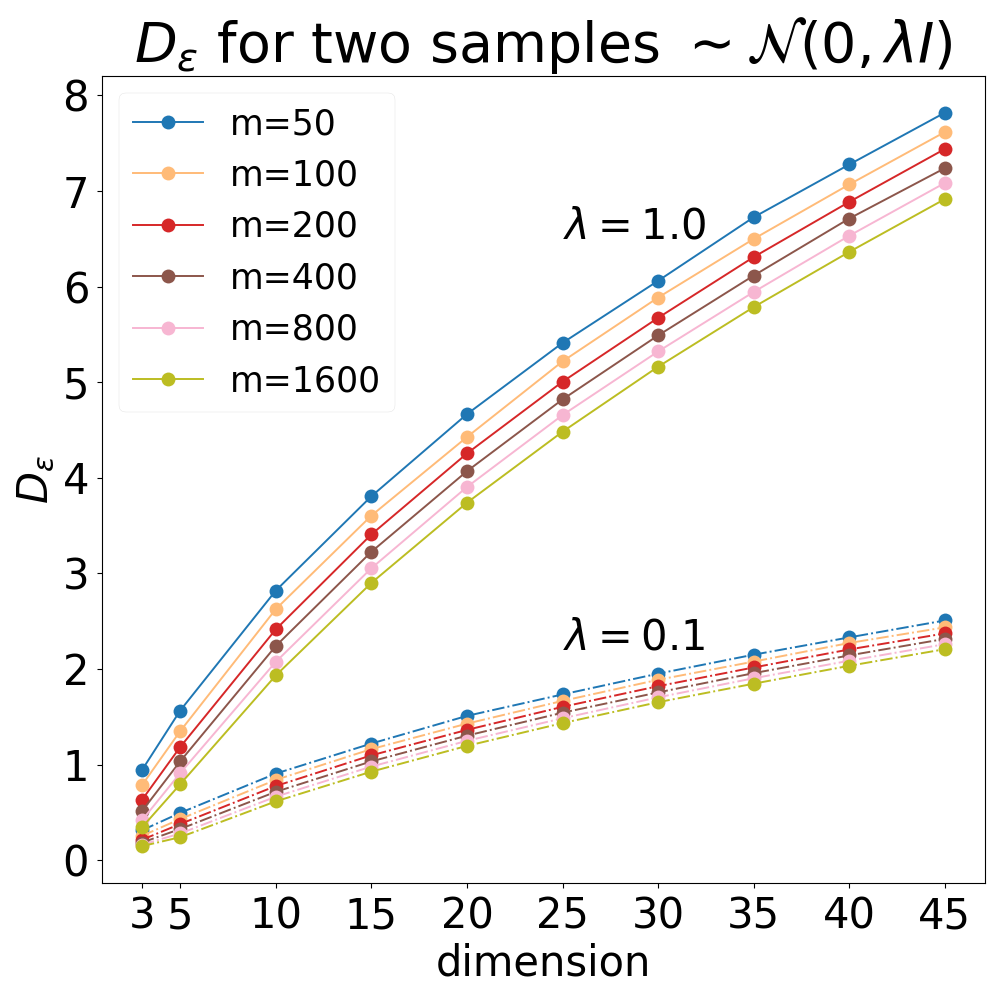
\includegraphics[width=0.8\columnwidth]{stability/plots/figures-EnKF-zeros_cov=0.1_cov=1.0.png}
\caption{Average $D_{\varepsilon}(\alpha_m^d, \beta_m^d)$ (over $20$ realizations) where $\alpha_m^d, \beta_m^d$ are two different sampling distributions with the same sample size $m$ for the same underlying $d$-dimensional Gaussian $\mathcal N(0_d, \lambda I_d)$}
\label{fig:plot-zeros--numerical-fs}
\end{figure}
In order to understand the convergence to $0$ of the above quantity [see~\eqref{eq-stablaw--numerical-fs}], we first discuss how close to zero $D_\varepsilon$ can approach numerically. In figure~\ref{fig:plot-zeros--numerical-fs} we see the average $D_\varepsilon(\alpha^d_m, \beta^d_m)$ where $\alpha_m^d=\frac{1}{m}\sum_{i=1}^m\delta_{x^{m,d}_i}$ and $\beta_m^d=\frac{1}{m}\sum_{i=1}^m\delta_{y^{m,d}_i}$, with $\{x^{m,d}_i\}$ and $\{y^{m,d}_i\}$ both samples from the same underlying $d$-dimensional Gaussian distribution $\mathcal N_d^\lambda:=\mathcal N(0_d, \lambda I_d)$. 
For `small' $\lambda$, we can expect $D_\varepsilon$ to behave in a similar fashion as if $\mathcal N_d^\lambda$ were supported on a compact set. With that in mind, we relate the numerical results shown in figure~\ref{fig:plot-zeros--numerical-fs} to the results~\ref{lem-prop--numerical-fs}--\ref{thm-zero--numerical-fs} in the appendix~\ref{sec-app--numerical-fs} by noting the following key points:

% By the phrase \textit{zero of the Sinkhorn algorithm} we mean the value of $D_\varepsilon$ obtained by using algorithm~\ref{algo-sink--numerical-fs} when the inputs are two different sampling distributions coming from the same underlying probability distribution.

\subsubsection{Drop with increase in sample size} Theorem~\ref{thm-zero--numerical-fs} explains the monotone drop in average $D_\varepsilon$ for a fixed dimension while increasing the sample size.

\subsubsection{Rise with increase in dimension} As the dimension increases, larger sample sizes are required to accurately estimate $\mathcal N_d^\lambda$. Consequently, $D_\varepsilon(\alpha_m^d, \beta_m^d)$ grows with $d$ for fixed $m$ since $\alpha_m^d, \beta_m^d$ become poorer estimators of $\mathcal N_d^\lambda$ as $d$ increases. 

 % PF 12 plots 
\begin{figure*}[!t]
\centering
\begin{subfigure}{0.3\textwidth}
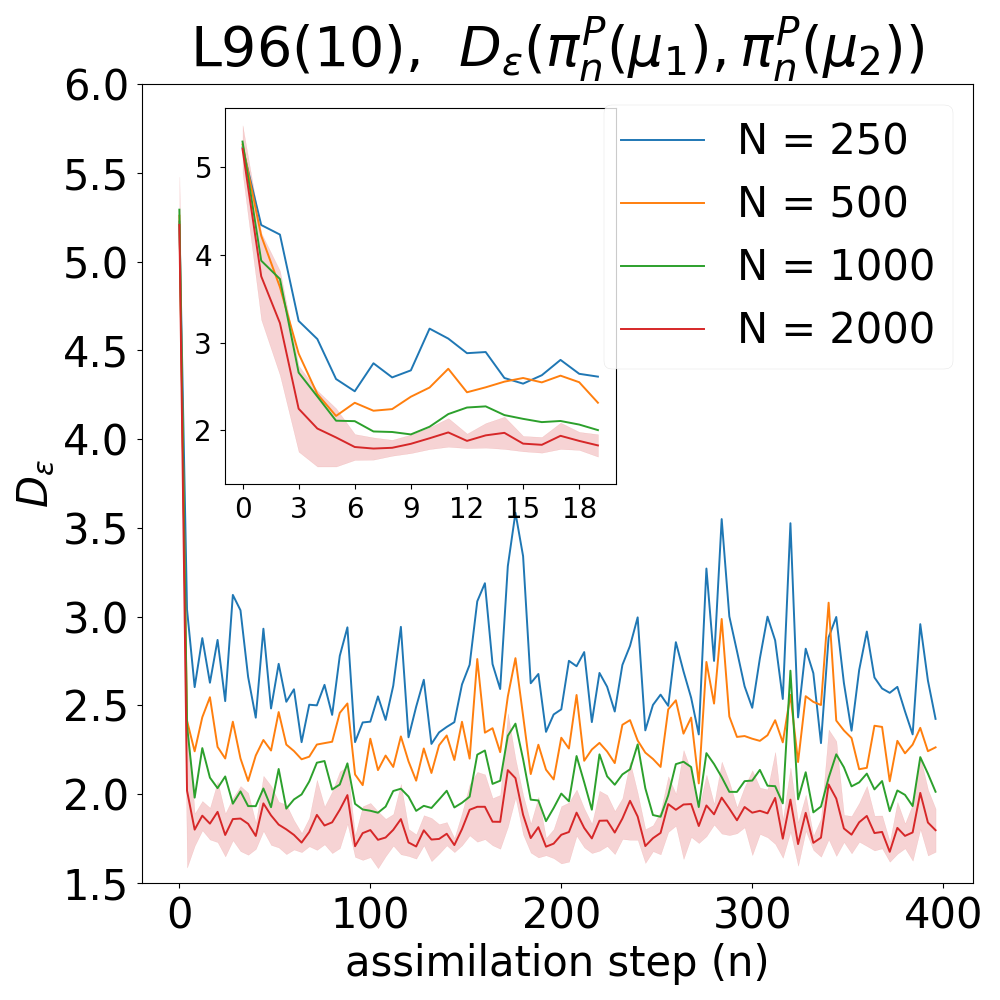
\includegraphics[width=\columnwidth]{stability/plots/figures-BPF-L96_10-1-dist_1_vs_2.png}
%\caption{dist 1 vs 2}
\end{subfigure}\hspace{0mm}%
\begin{subfigure}{0.3\textwidth}
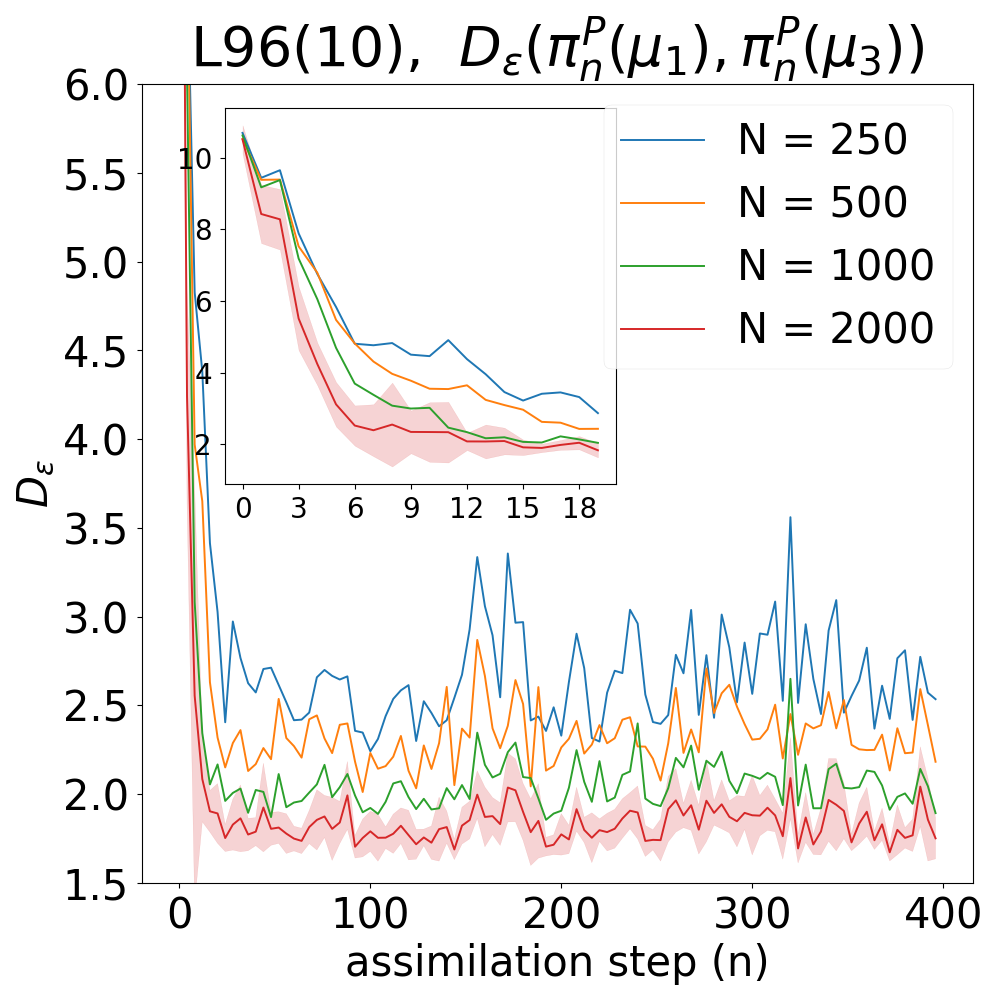
\includegraphics[width=\columnwidth]{stability/plots/figures-BPF-L96_10-1-dist_1_vs_3.png}
%\caption{dist 1 vs 3}
\end{subfigure}\hspace{0mm}%
\begin{subfigure}{0.3\textwidth}
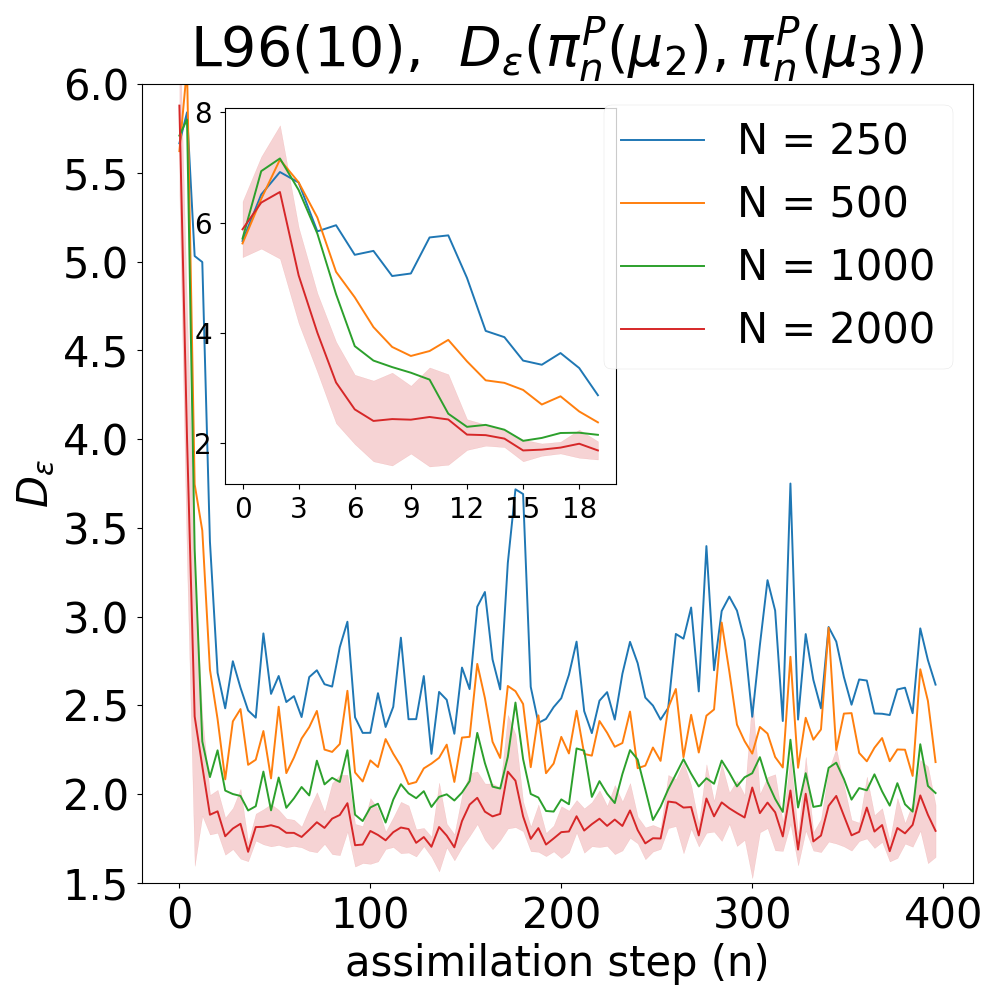
\includegraphics[width=\columnwidth]{stability/plots/figures-BPF-L96_10-1-dist_2_vs_3.png}
%\caption{dist 2 vs 3}
\end{subfigure}\hspace{0mm}%

\begin{subfigure}{0.3\textwidth}
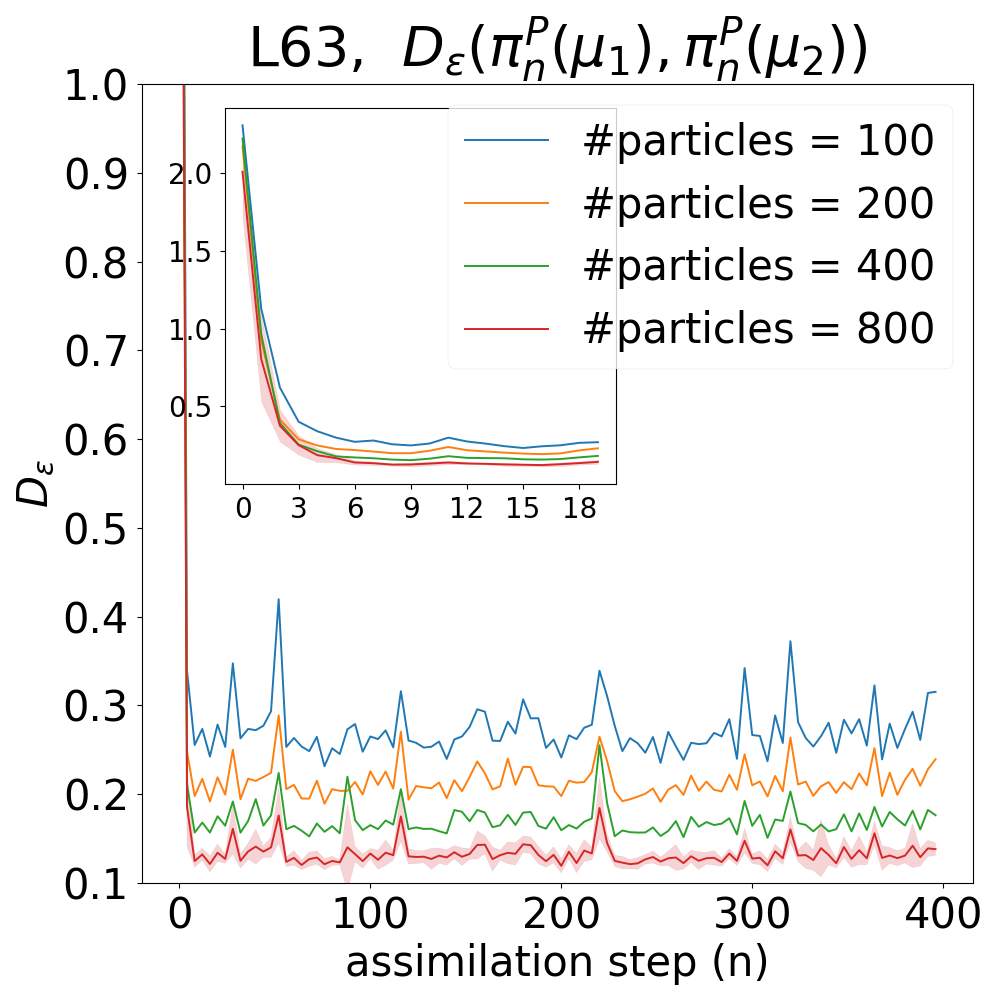
\includegraphics[width=\columnwidth]{stability/plots/figures-BPF-L63-1-dist_1_vs_2.png}
%\caption{dist 1 vs 2}
\end{subfigure}\hspace{0mm}%
\begin{subfigure}{0.3\textwidth}
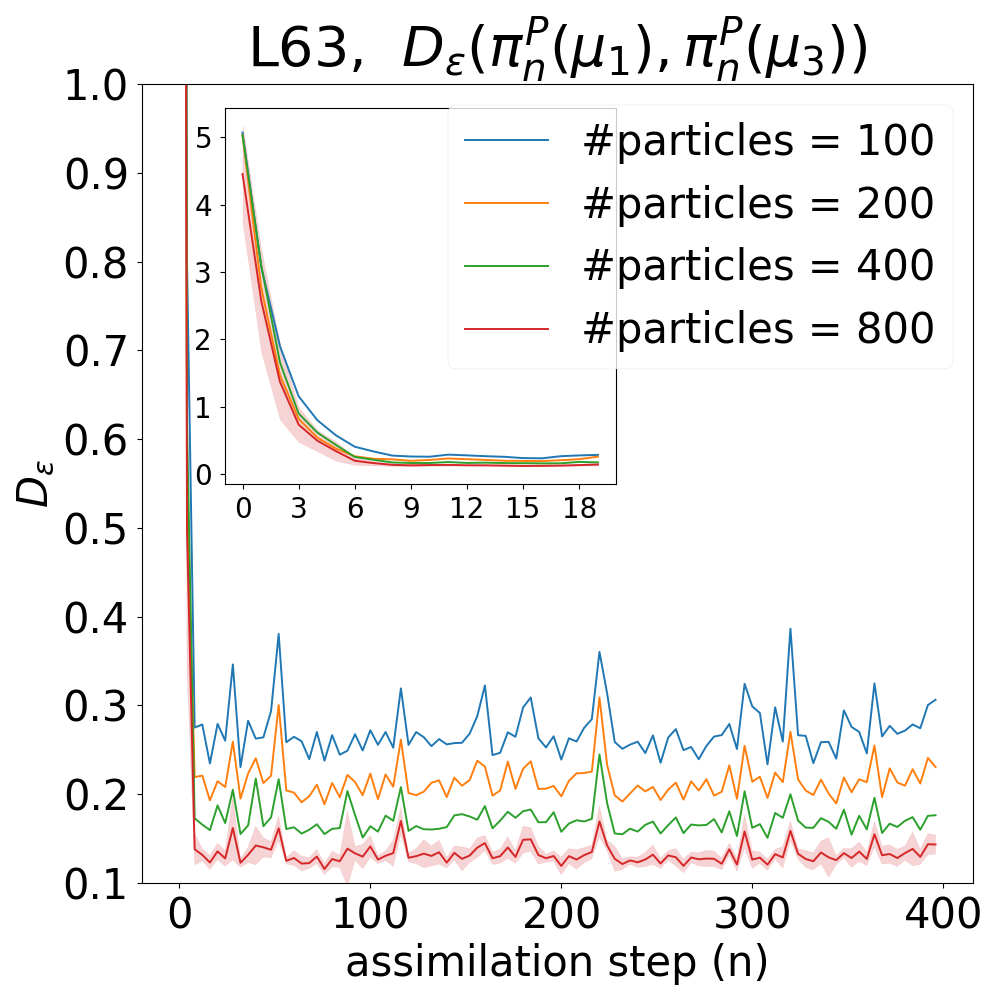
\includegraphics[width=\columnwidth]{stability/plots/figures-BPF-L63-1-dist_1_vs_3.png}
%\caption{dist 1 vs 3}
\end{subfigure}\hspace{0mm}%
\begin{subfigure}{0.3\textwidth}
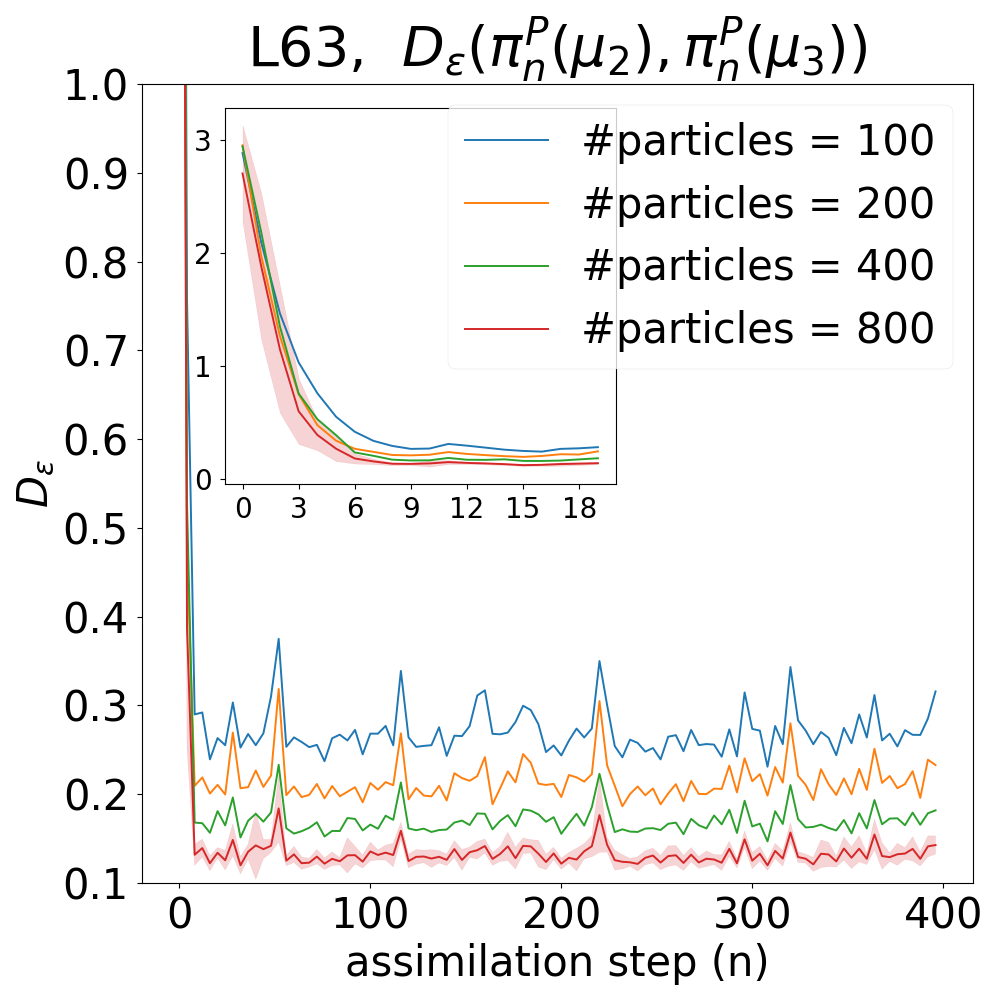
\includegraphics[width=\columnwidth]{stability/plots/figures-BPF-L63-1-dist_2_vs_3.png}
%\caption{dist 2 vs 3}
\end{subfigure}\hspace{0mm}
\caption{$D_\varepsilon$ (averaged over $10$ observation realizations) for BPF for $10$-dimensional $L96$ (row 1) and $L63$ (row 2) systems with observation covariance $\sigma^2=0.1$, for pairs of initial distributions in~\eqref{eq-3ic--numerical-fs}, with varying sample size. The line for $N = 2000$ has a band showing one standard deviation. The inset shows the drop in average $D_\varepsilon$ during the first few assimilation steps.}
\label{fig:plot-BPF--numerical-fs}
\end{figure*}

\subsubsection{Drop with decrease in covariance} Decreasing the covariance $\lambda$ has the opposite effect since, for fixed dimension $d$ and sample size $m$, smaller covariance leads to a better estimation of the underlying distribution, i.e., $\alpha_m^d, \beta_m^d$ become better estimators of $\mathcal N_d^\lambda$ as $\lambda$ decreases.

\subsubsection{Support of our distributions} Since the true trajectories for both systems (L63, L96) lie on bounded attractors, we can assume that true filtering distributions are supported on a compact set. Consequently, in the filtering experiments shown later, the zero of the Sinkhorn algorithm shows qualitatively similar behavior (e.g., in figure~\ref{fig:plot-BPF--numerical-fs}) with respect to dimension as seen in figure~\ref{fig:plot-zeros--numerical-fs}.

\subsection{Particle Filter}
Here we use the notation $\pi^{P, N}_n$ for $\hat\pi_n$ obtained by alogithm~\ref{algo-bpf--numerical-fs} with $N$ particles (omitting $N$ for brevity when value of $N$ is clear from context). Figure~\ref{fig:plot-BPF--numerical-fs} shows $\mathbb E[D_\varepsilon(\hat\pi_n(\mu_i), \hat\pi_n(\mu_j))], \ i \ne j$ as a function of $n$. We note some important conclusions.
\subsubsection{BPF quickly forgets the initial distribution} From the insets in figure~\ref{fig:plot-BPF--numerical-fs} we can see that for every pair $(\mu_i, \mu_j)$ of initial distributions, $\mathbb E\left[D_\varepsilon(\pi^P_n(\mu_i), \pi^P_n(\mu_j))\right]$ stabilizes in the first few assimilation steps. In fact, this behavior is consistent with exponential stability of particle filters \cite{chigansky2009intrinsic}.
\subsubsection{Dependence on the number of particles} 
$\mathbb E\left[D_\varepsilon(\pi^{P, N}_n(\mu_i), \pi^{P, N}_n(\mu_j))\right]$ for a fixed $n$ decreases monotonically with increasing $N$ for both L63 and L96 and for both observation covariances for all pairs $i\neq j$.
%$\pi^{P,N}_n$ weak$^*$ converges to the true filtering distribution $\pi_n$ as $N\to\infty$ \cite{van2008hidden}. This fact along with theorem \ref{thm-zero--numerical-fs} is enough for explaining the drop in $D_\varepsilon$ in figure~\ref{fig:plot-BPF--numerical-fs} for fixed $n$ as we increase $N$.
\subsubsection{Stability}
Suppose the best possible filtering distribution that can be computed by the particle filter is $\pi^{P,*}_n=\lim_{N\to\infty}\pi^{P,N}_n$. Figure~\ref{fig:plot-BPF--numerical-fs} is consistent with the condition
\begin{align*}
    \lim_{n\to\infty}\liminf_{N\to\infty}\mathbb E[D_\varepsilon(\pi^{P,N}_n(\mu_i), \pi^{P,N}_n(\mu_j))]=0\;\forall\; i\neq j
\end{align*}
since fixing $n$ and increasing $N$ results in a steady drop in $D_\varepsilon$ averaged over observation realizations. By theorem \ref{thm-stable--numerical-fs} this condition is sufficient for concluding
\begin{align*}
    \lim_{n\to\infty}\mathbb E[D_\varepsilon(\pi^{P,*}_n(\mu_i), \pi^{P,*}_n(\mu_j))]=0\;\forall\; i\neq j
\end{align*}
\subsubsection{Dependence on observation covariance} All plots in figure~\ref{fig:plot-BPF--numerical-fs} correspond to observation covariance $\sigma^2=0.1$. The other case $\sigma^2=1.0$ mentioned in \ref{ssec-models--numerical-fs} results in plots that are qualitatively similar to the ones in figure~\ref{fig:plot-BPF--numerical-fs} and we omit those plots here. In our experiments, stability of particle filter was not seen to be affected by observation covariance. 

\subsection{EnKF}
% Enkf 3 plot, 1 is left:
\begin{figure*}[!t]
\centering
\begin{subfigure}{.3\textwidth}
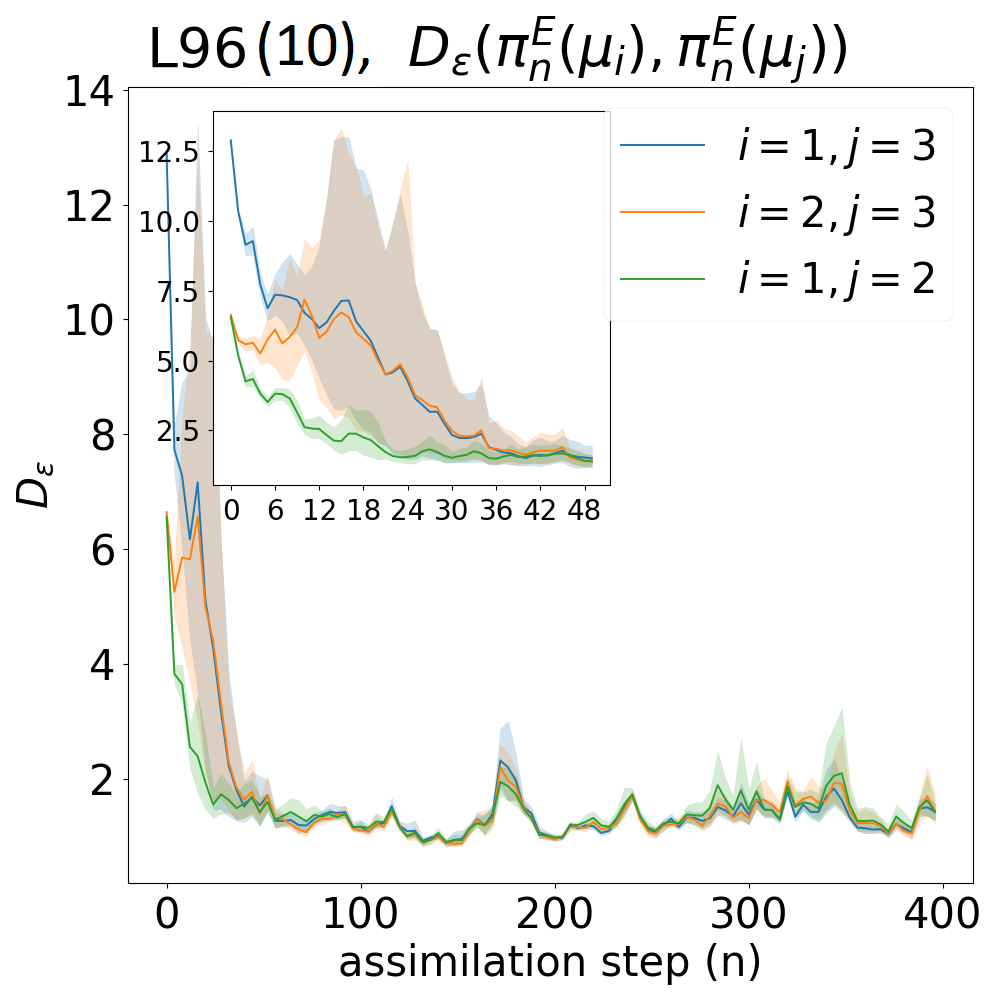
\includegraphics[width=\columnwidth]{stability/plots/figures-EnKF-stable_50_L96_10dim.png}%
%\caption{N=50 with localization}%
%\label{sub@fig:plot-enkf50--numerical-fs}%
\end{subfigure}\hspace{0mm}% 
\begin{subfigure}{.3\textwidth}
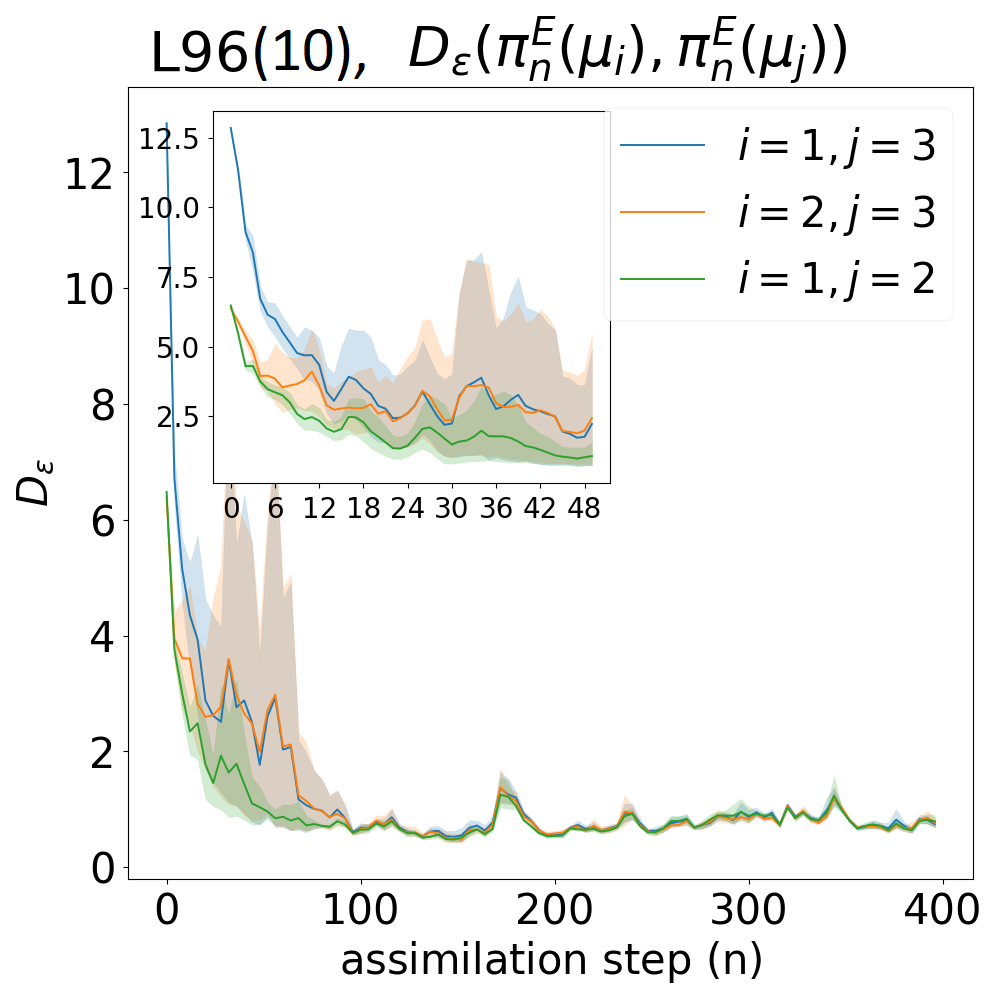
\includegraphics[width=\columnwidth]{stability/plots/figures-EnKF-stable_200_L96_10dim.png}%
%\caption{N=200 without localization}%
%\label{sub@fig:plot-enkf200--numerical-fs}%
\end{subfigure}\hspace{0mm}%
\begin{subfigure}{.3\textwidth}
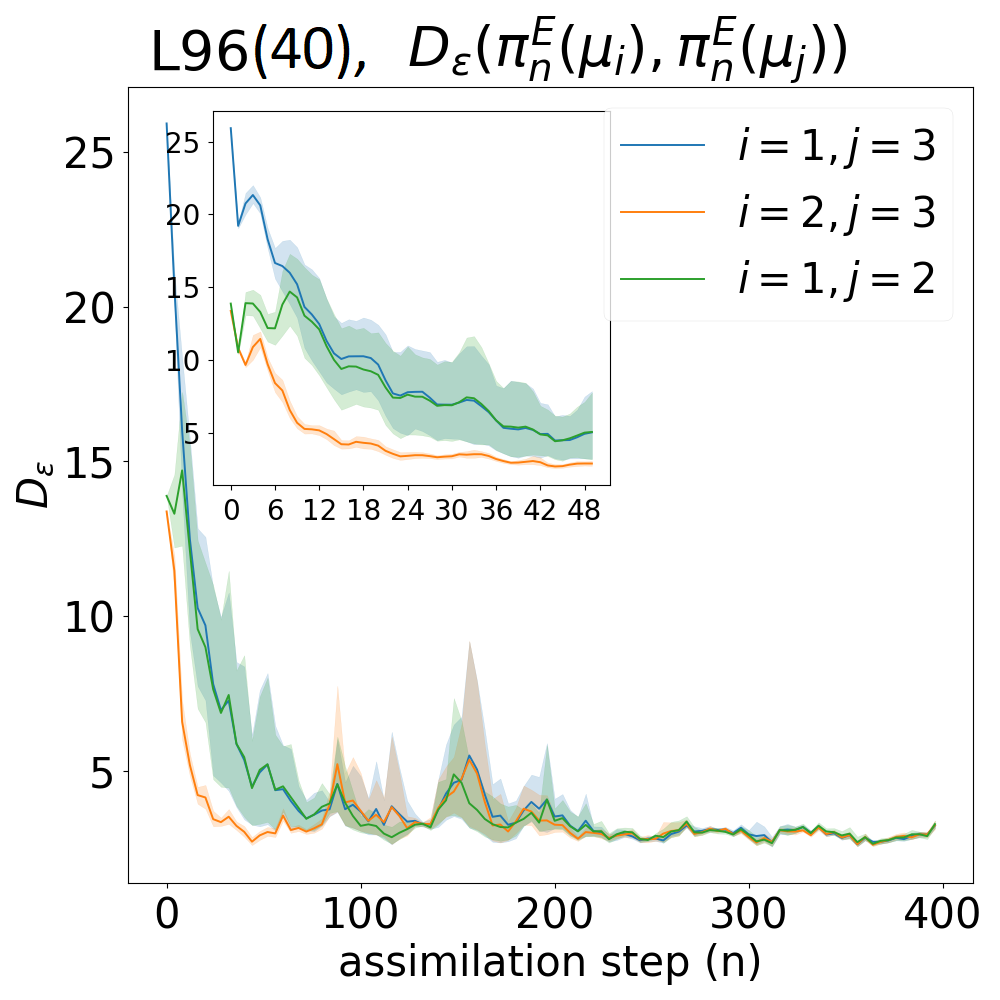
\includegraphics[width=\columnwidth]{stability/plots/figures-EnKF-stable_50_loc_L96_40dim.png}%
%\caption{$D_\varepsilon$ for $\mu_{i}$ with N=50,200}%
%\label{sub@fig:plot-enkfL96-40--numerical-fs}%
\end{subfigure}%
\caption{$D_\varepsilon$ (averaged over $10$ observation realizations, with one standard deviation confidence band) for EnKF for $10$-dimensional L96 with $N=50$ with localization (left), $N=200$ without localization (middle) for observation covariance $\sigma^2=0.1$, and for $40$-dimensional L96 with $N=50$ with localization (right) with observation covariance $\sigma^2=1.0$ for pairs of initial distributions in \ref{eq-3ic--numerical-fs}. The inset shows the drop in $D_\varepsilon$ for the first 50 assimilation steps.}
\label{fig:plot-enkfL96-10--numerical-fs}
\end{figure*}
Here we use the notation $\pi^{E,N}_n$ for $\hat\pi_n$ obtained by alogithm~\ref{algo-enkf--numerical-fs} with ensemble size $N$. We might omit $N$ for brevity.
\subsubsection{Drop in $D_\varepsilon$ over time}
From figure~\ref{fig:plot-enkfL96-10--numerical-fs}, we see that for every pair $(\mu_i, \mu_j)$ of initial distributions $D_\varepsilon(\pi^E_n(\mu_i), \pi^E_n(\mu_j))$ decreases with time rapidly within the first $50$ assimilation steps and beyond $100$ assimilation steps, the observation average of $D_\varepsilon$ for filters with different pairs initial distributions are similar and have very little variance.
\subsubsection{Variation with respect to observation realization} We see that the variation of $D_\varepsilon$ for different observation realizations (shown by the shaded bands in left two panels in figure~\ref{fig:plot-enkfL96-10--numerical-fs} and in top row in figure~\ref{fig:plot-BPF--numerical-fs}) is larger for the case of EnKF when compared to the particle filter for initial times (e.g. $n < 100$ for the 10-dimensional L96 model). On the other hand, for larger times (approx.~$n > 100$), the variation for EnKF is significantly smaller than the particle filter.
% \subsubsection{}
% For $10$-dimensional L96 system, we see that the $D_\varepsilon$ between the filer with localization and without localization for the same initial distribution are different but stable.  
\subsubsection{Effect of localization}
EnKF with small ensemble size needs localization which, however, is an ad-hoc procedure to prevent filter divergence and may not approximate the true filter. Figure~\ref{fig:plot-enkfL96-10--numerical-fs} for $10$-dimensional L96 (left panel) and for $40$-dimensional L96 (right panel) shows that for $N=50$ with localization length 4, the EnKF is stable, whereas the middle panel shows the stability (with the same configuration as the left panel) for $10$-dimensional L96 without localization, but with larger ensemble size $N=200$. This indicates that that localization does not affect EnKF's stability properties.

% L96-40 dimensions plot
% \begin{figure}
% \centering
% 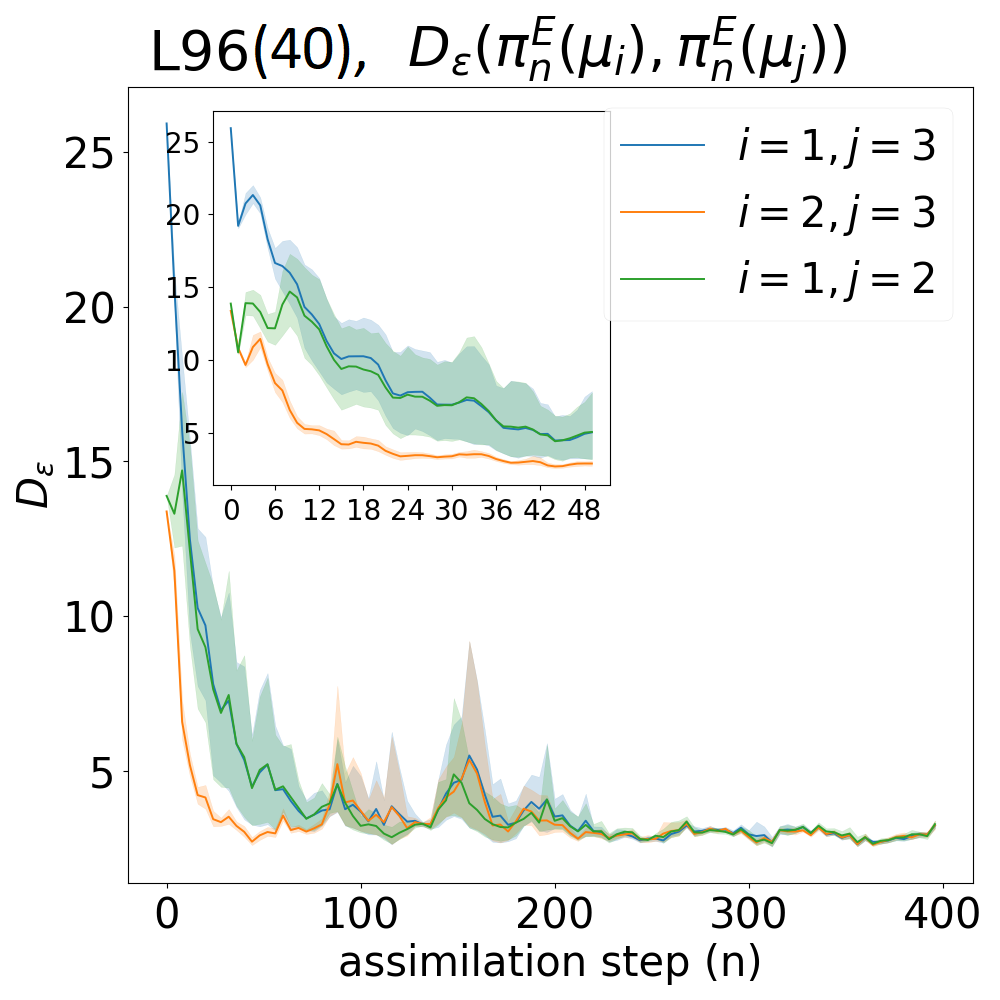
\includegraphics[width=0.8\columnwidth]{stability/plots/figures-EnKF-stable_50_loc_L96_40dim.png}
% \caption{$D_\varepsilon$ for $40$-dimensional L96 model for N=50 with localization length=4.}
% \label{fig:plot-enkfL96-40--numerical-fs}
% \end{figure}

\subsection{BPF vs EnKF}
\begin{figure}
\centering
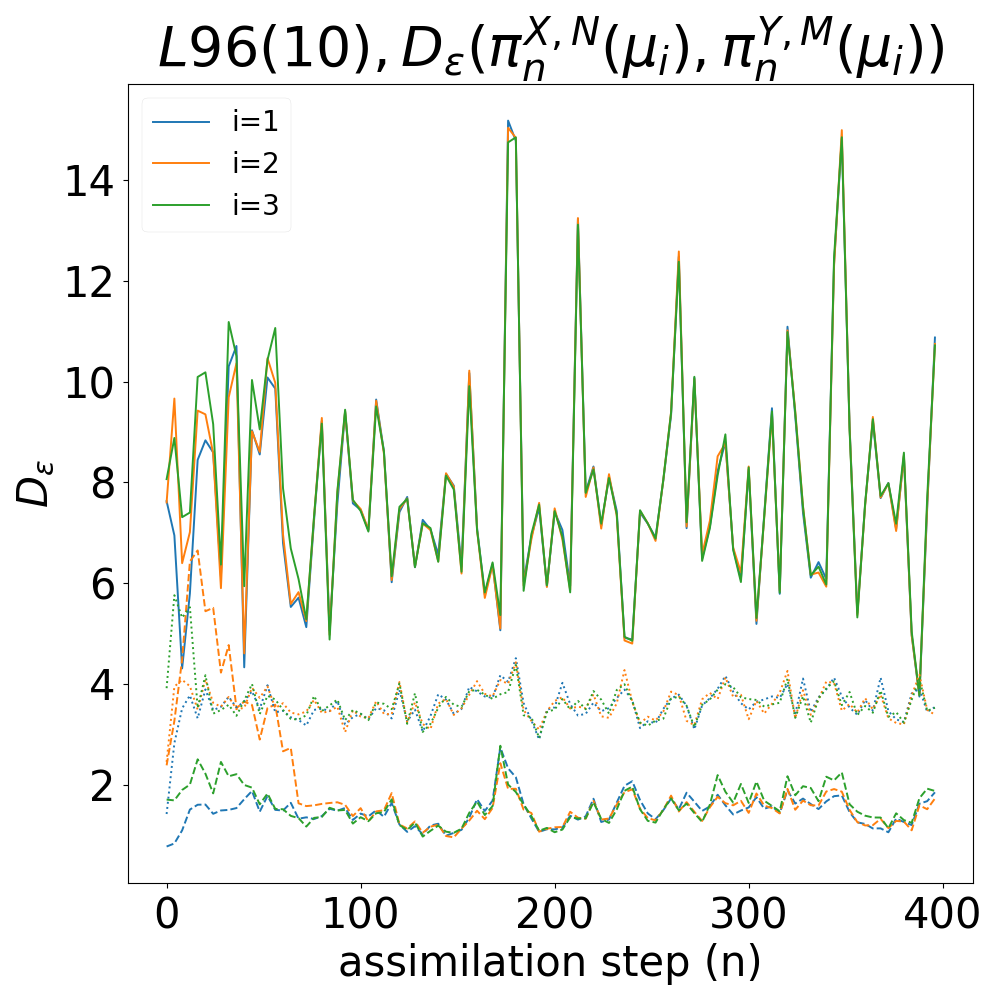
\includegraphics[width=0.8\columnwidth]{stability/plots/figures-BPF-L96_10-EnKF-distance between different filters.png}
\caption{Comparison between filters for $10$-dimensional L96 and $\sigma^2=1.0$. The solid lines on the top show average $D_\varepsilon$ between EnKF without localization with $N = 200$ and BPF with $M = 2000$. The dotted lines in the middle show average  $D_\varepsilon$ between  BPF with $N = 250$ and BPF with $M = 2000$. The dashed lines at the bottom show average  $D_\varepsilon$ between EnKF without localization with $N = 200$ and EnKF with localization with $M = 50$. In each case, different colors are for different initial conditions from~\eqref{eq-3ic--numerical-fs}.} 
\label{fig:plot-compare--numerical-fs}
\end{figure}
We now compare the BPF and EnKF for the case of $10$-dimensional L96 with $\sigma^2=1.0$ with the same true trajectory and observation realizations. This is shown in figure~\ref{fig:plot-compare--numerical-fs}. {In the following discussion we assume BPF with 2000 particles to be a decent approximation for the true filter and refer to them interchangably.} We note a few important points.
\subsubsection{Poor approximation of the true filter by EnKF} The three lines towards the top show the distance between EnKF and BPF, for three different initial conditions. We see that EnKF produces distributions that are significantly different from the true filter, for all the initial distributions. But recall that for this setup, the EnKF is stable (as is the BPF too), i.e., the distance between EnKF with different initial conditions is smaller (as seen in figures~\ref{fig:plot-BPF--numerical-fs}-\ref{fig:plot-enkfL96-10--numerical-fs}) than the distance between the BPF and EnKF
\subsubsection{BPF is closer to the true filter than is EnKF} The three lines in the middle show the distance between BPF with $N=250$ and $N=2000$ (putatively true filter). We see that in comparison with EnKF with $N=200$ particles, BPF with similar ensemble size (250 particles) is much closer to the true filter.
\subsubsection{EnKF with different ensemble size are very similar} The bottom three lines in figure~\ref{fig:plot-compare--numerical-fs} show $D_\varepsilon$ between EnKF with different ensemble size, which shows that the EnKF is quite stable with respect to changes in the ensemble size, even though it is not very close to the true filter -- thus EnKF is stable but biased, whereas BPF is stable and unbiased. A more detailed study of the reasons for this behaviour will be taken up in the future.

% %trial and all error : this is to be removed.
% \begin{figure*}
% \centering
% %\begin{tabular}{ccc}
% \subcaptionbox{caption\label{1--numerical-fs}}{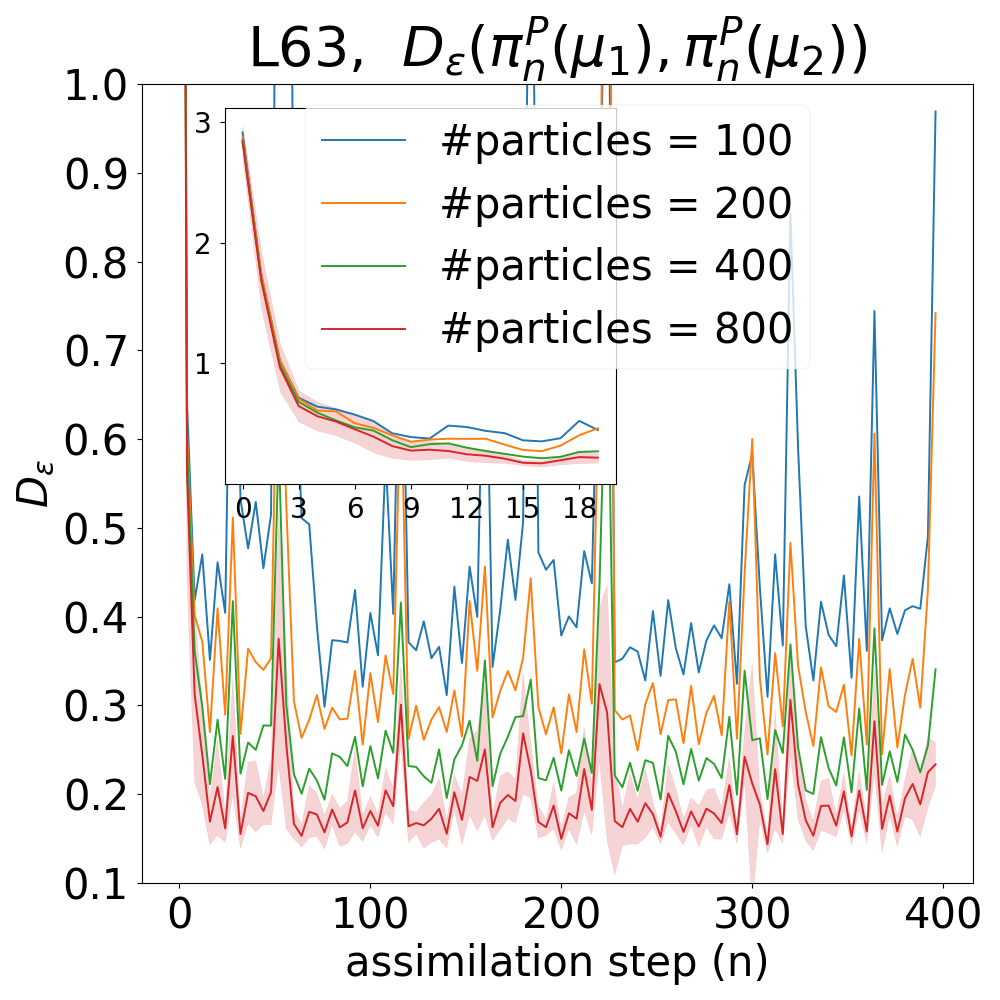
\includegraphics[width=0.28\textwidth]{stability/plots/figures-BPF-L63-0-dist_1_vs_2.png}}\hspace{0mm}
% \subcaptionbox{caption\label{2--numerical-fs}}{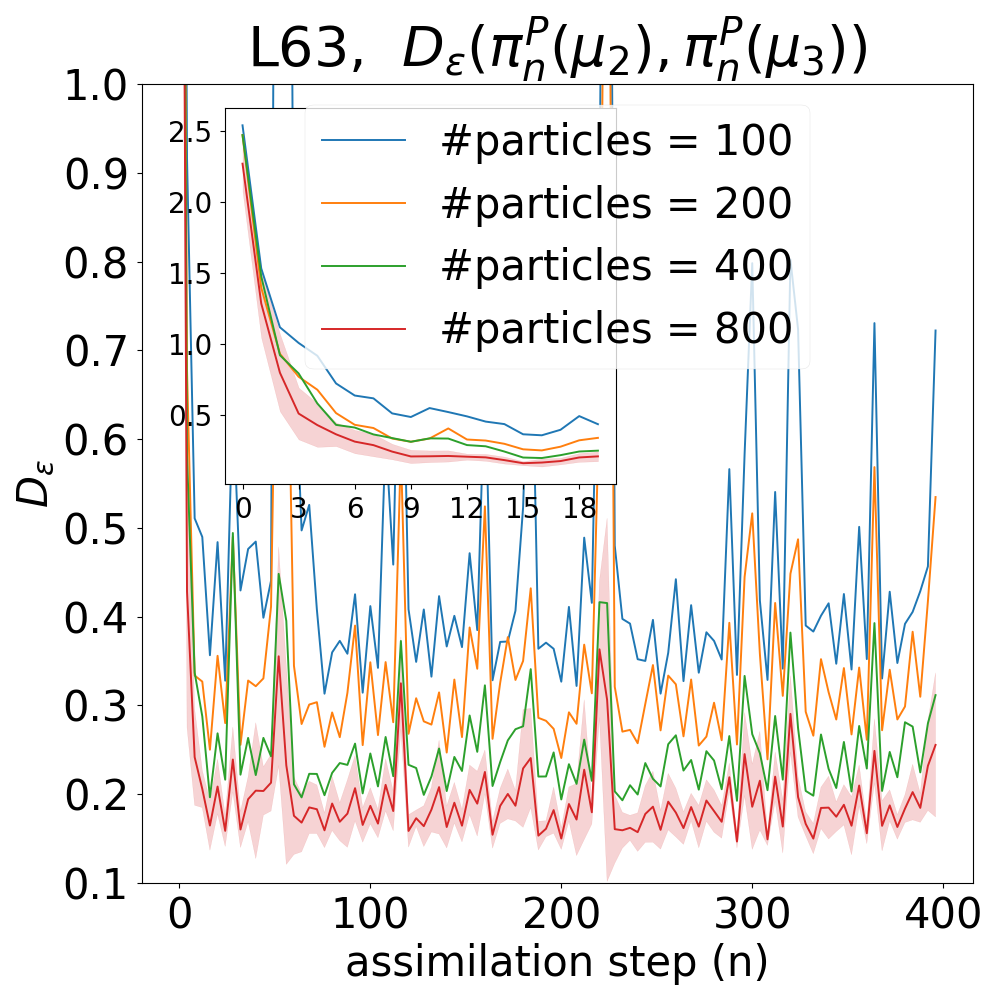
\includegraphics[width =0.28\textwidth]{stability/plots/figures-BPF-L63-0-dist_2_vs_3.png}}\hspace{0mm}
% \subcaptionbox{caption\label{2--numerical-fs}}{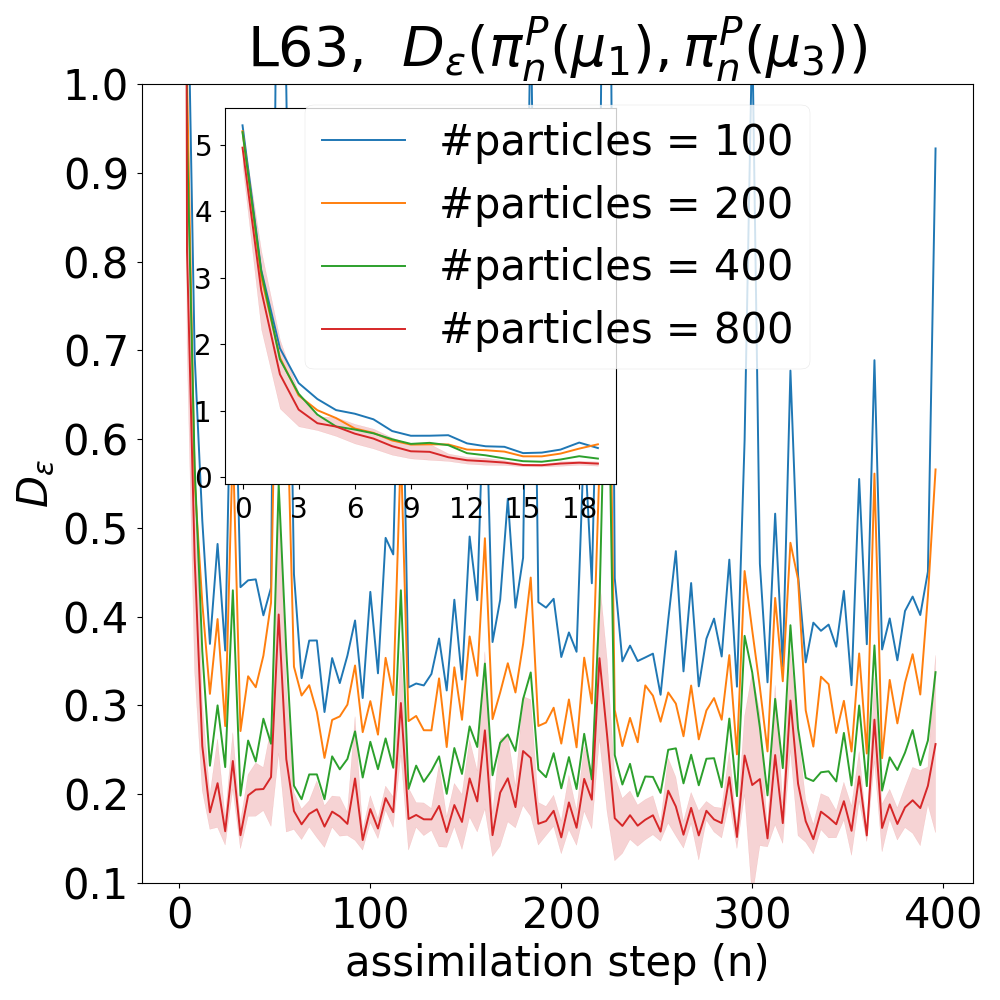
\includegraphics[width = 0.28\textwidth]{stability/plots/figures-BPF-L63-0-dist_1_vs_3.png}}\hspace{0mm}//%
% \subcaptionbox{caption\label{1--numerical-fs}}{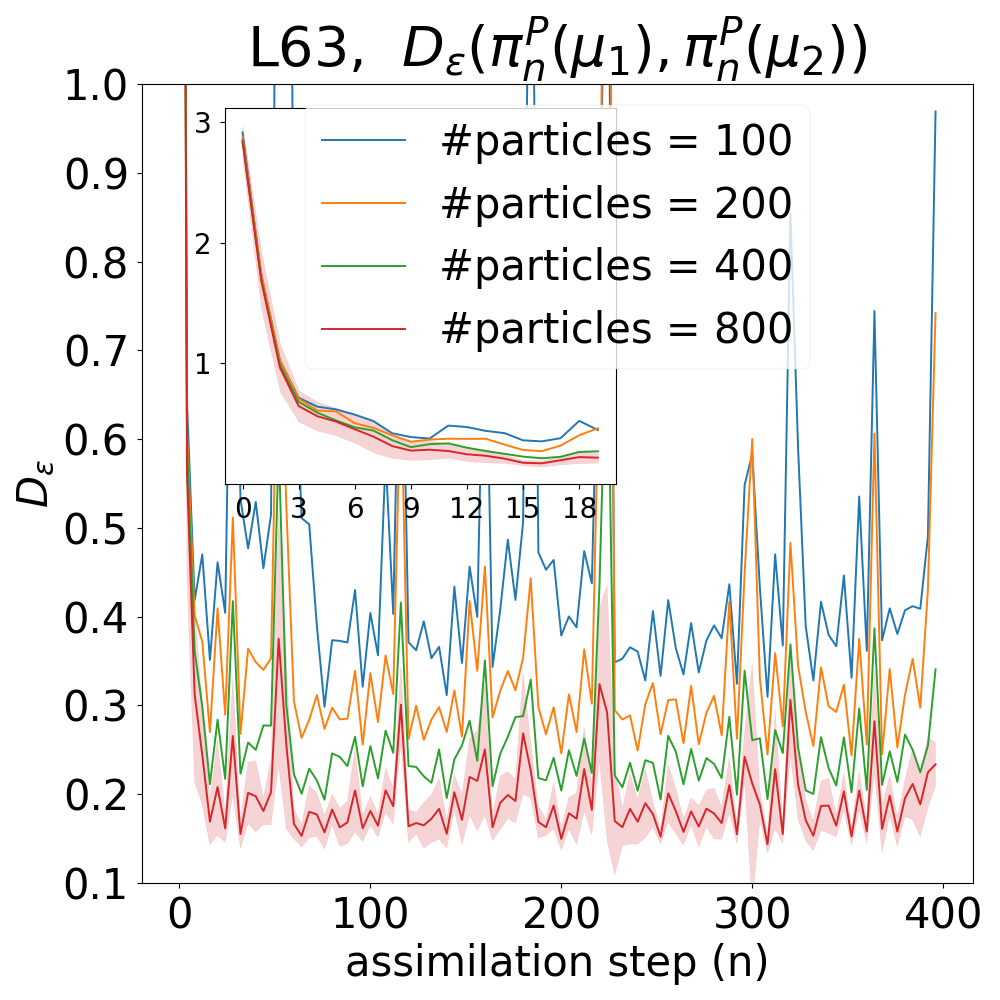
\includegraphics[width=0.28\textwidth]{stability/plots/figures-BPF-L63-0-dist_1_vs_2.png}}\hspace{0mm}
% \subcaptionbox{caption\label{2--numerical-fs}}{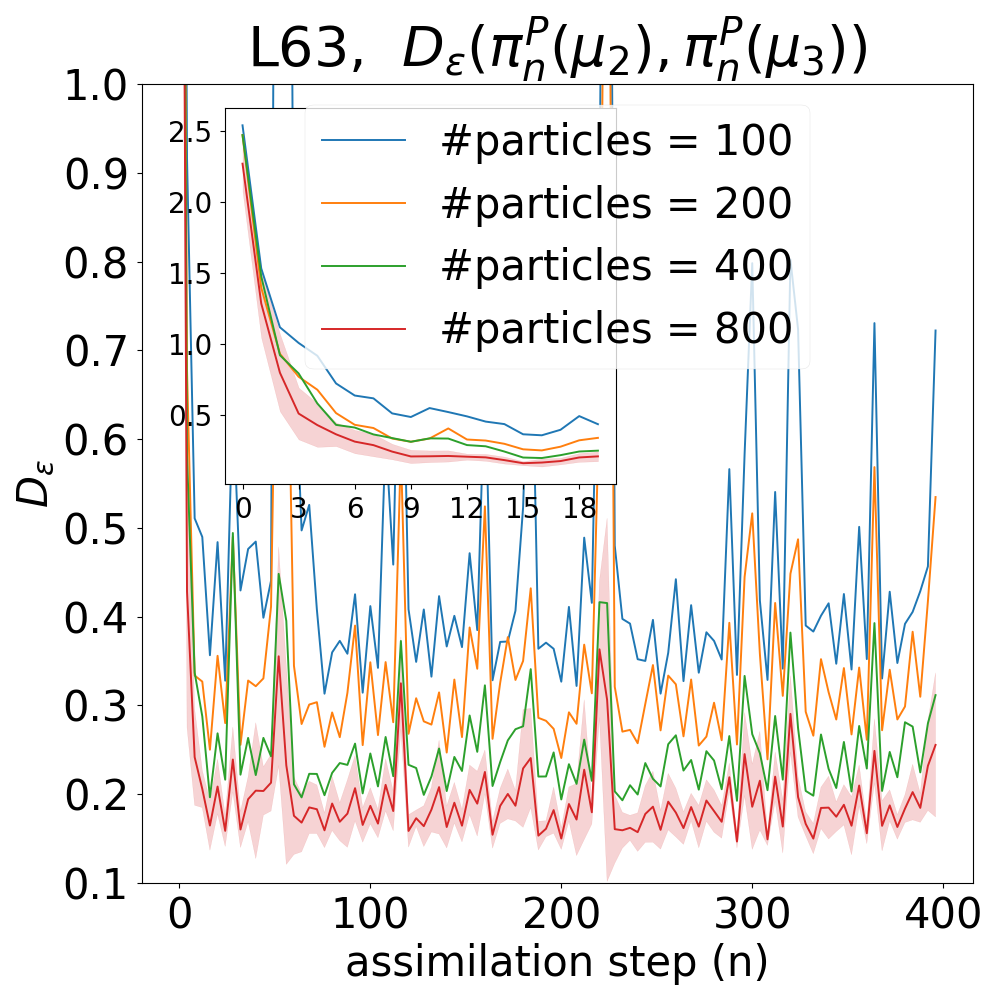
\includegraphics[width =0.28\textwidth]{stability/plots/figures-BPF-L63-0-dist_2_vs_3.png}}\hspace{0mm}
% \subcaptionbox{caption\label{2--numerical-fs}}{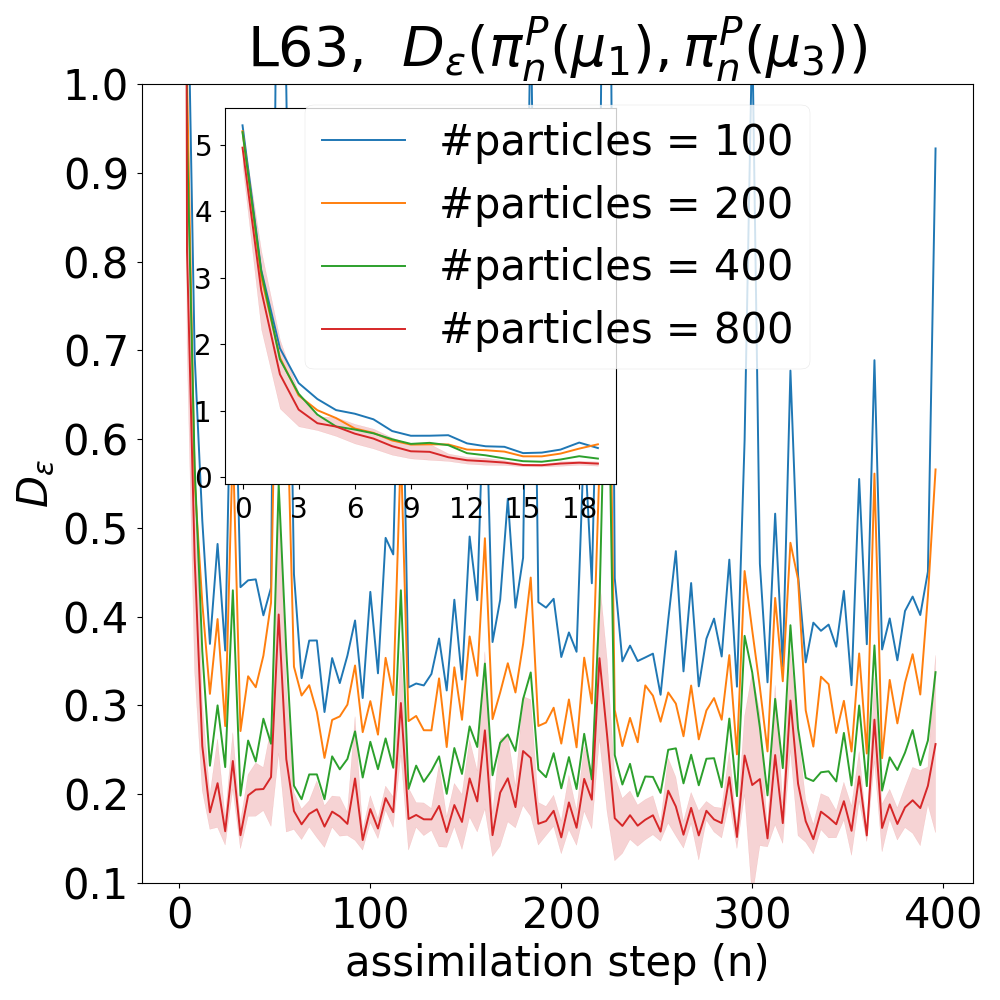
\includegraphics[width = 0.28\textwidth]{stability/plots/figures-BPF-L63-0-dist_1_vs_3.png}}\hspace{0mm}//
% %\end{tabular}
% \caption{caption}
% \label{fig2--numerical-fs}
% \end{figure*}

% \begin{figure*}[p]
% \begin{tabular}{c|c|c|c}

% {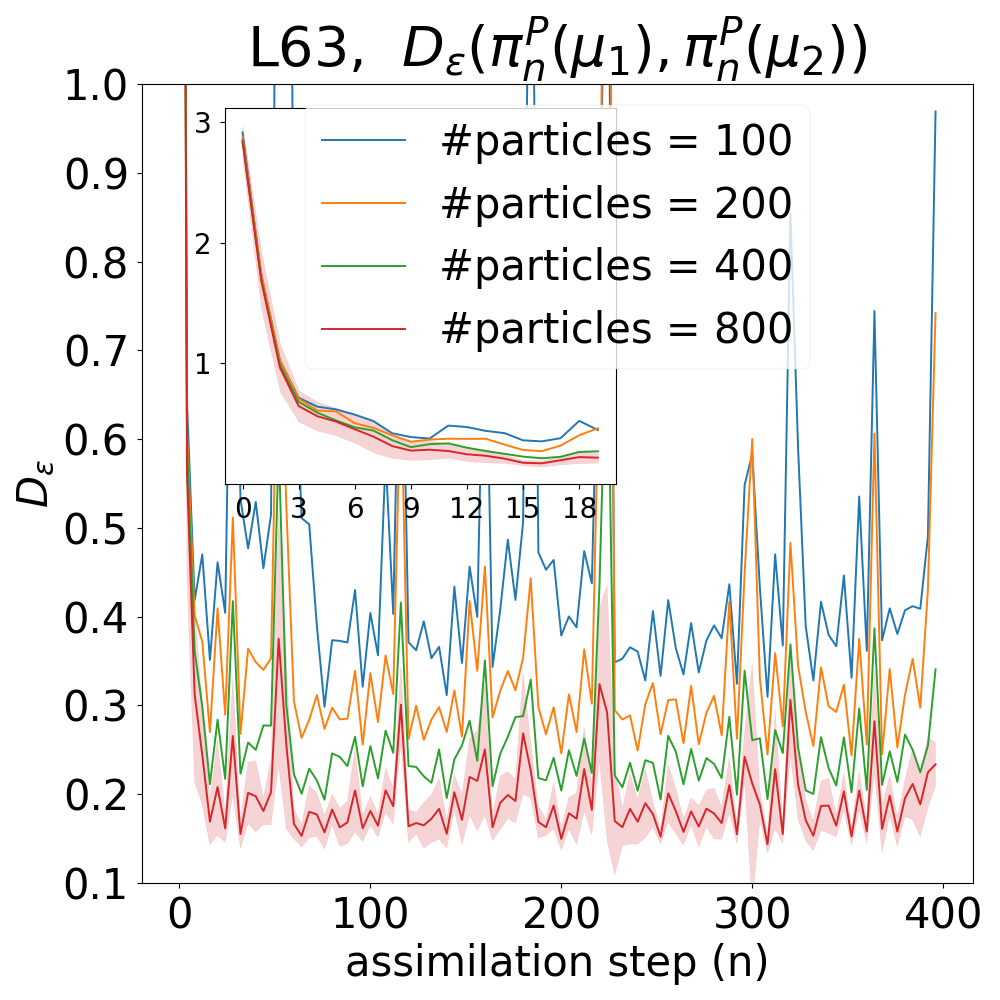
\includegraphics[width=0.2\textwidth]{stability/plots/figures-BPF-L63-0-dist_1_vs_2.png}} &
% {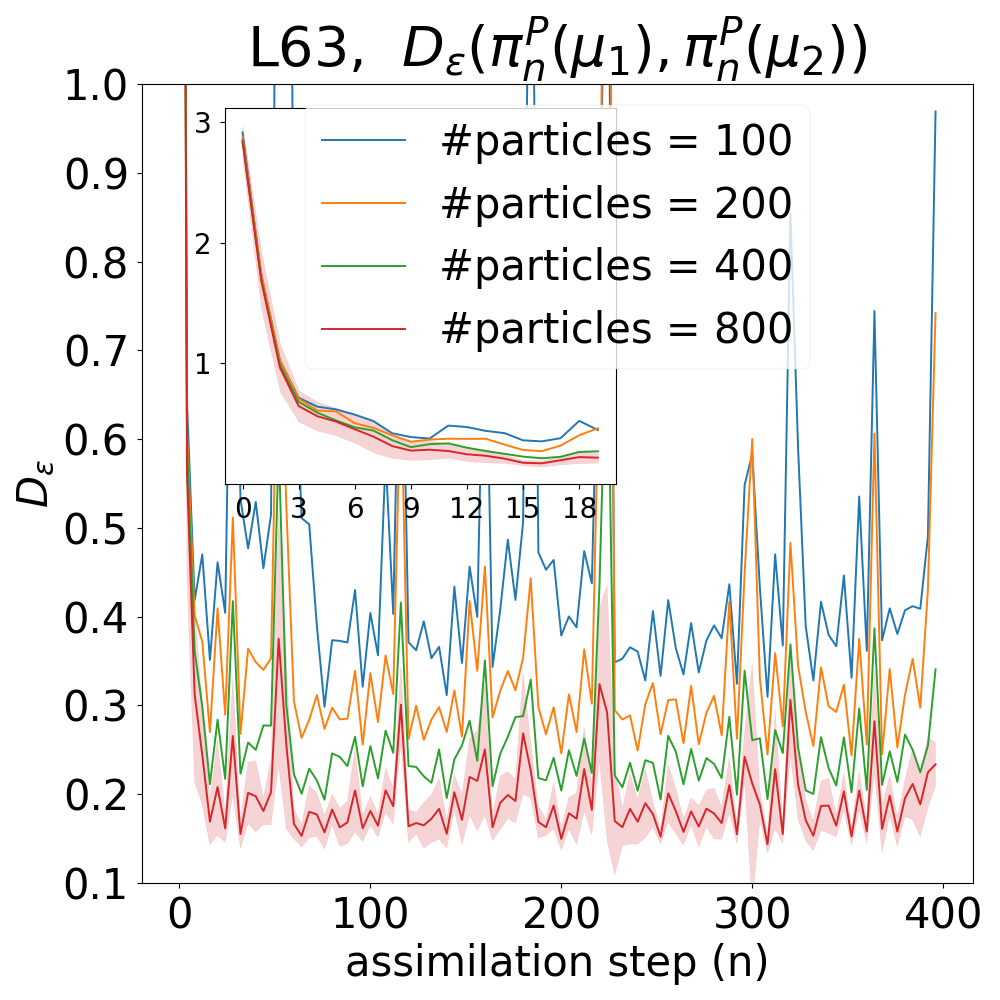
\includegraphics[width=0.2\textwidth]{stability/plots/figures-BPF-L63-0-dist_1_vs_2.png}} &
% {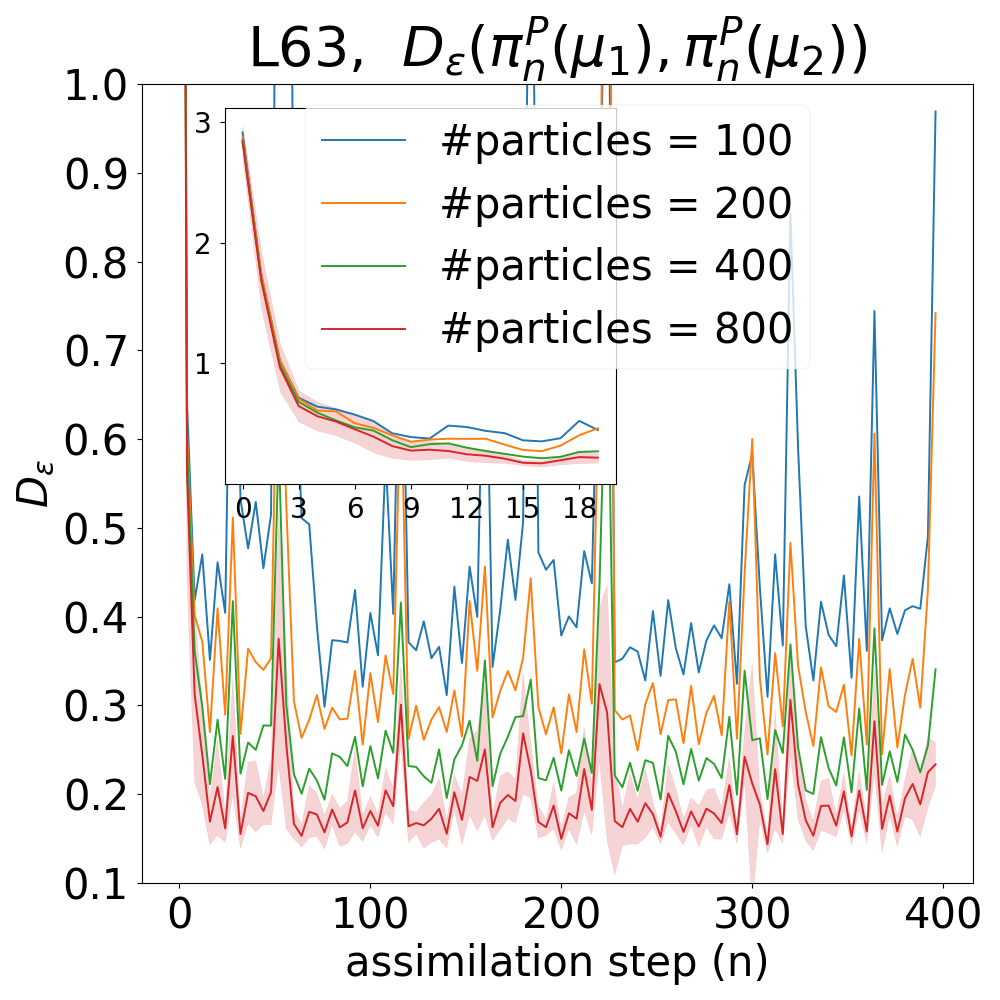
\includegraphics[width=0.2\textwidth]{stability/plots/figures-BPF-L63-0-dist_1_vs_2.png}} \\

% {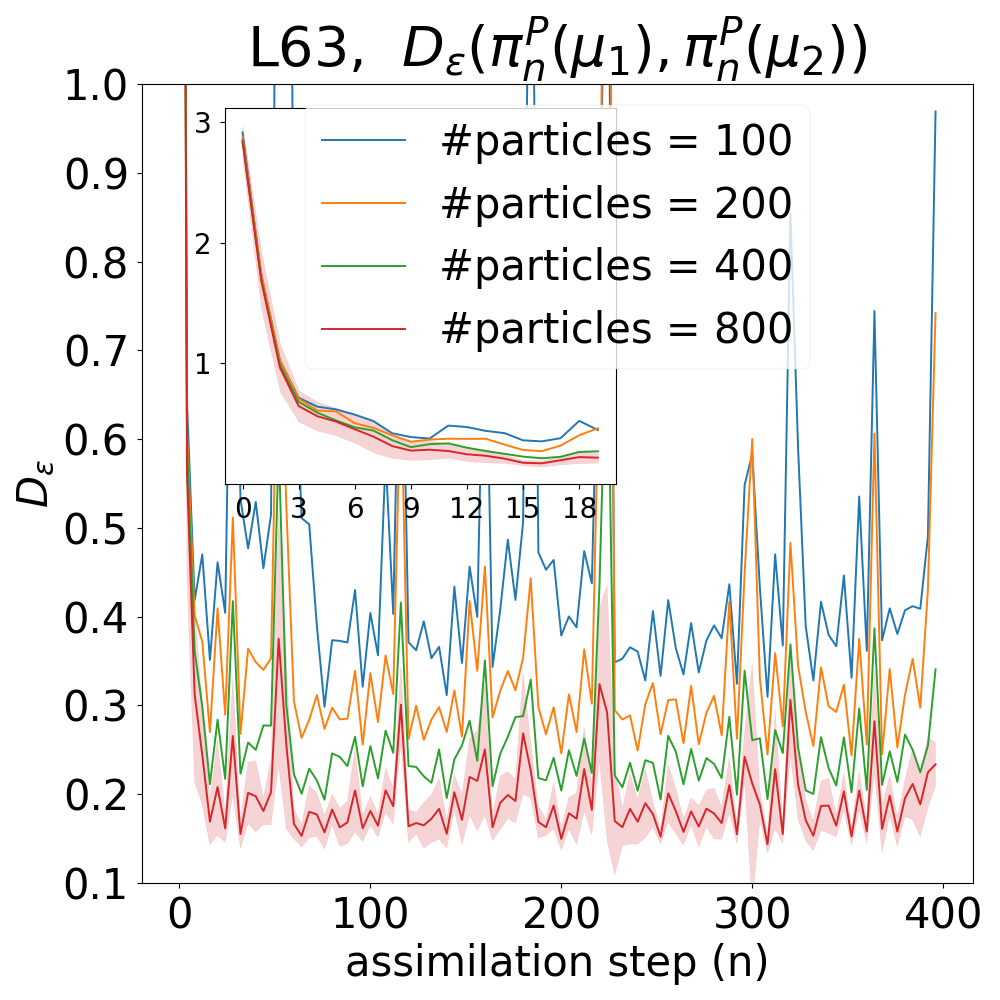
\includegraphics[width=0.2\textwidth]{stability/plots/figures-BPF-L63-0-dist_1_vs_2.png}} &
% {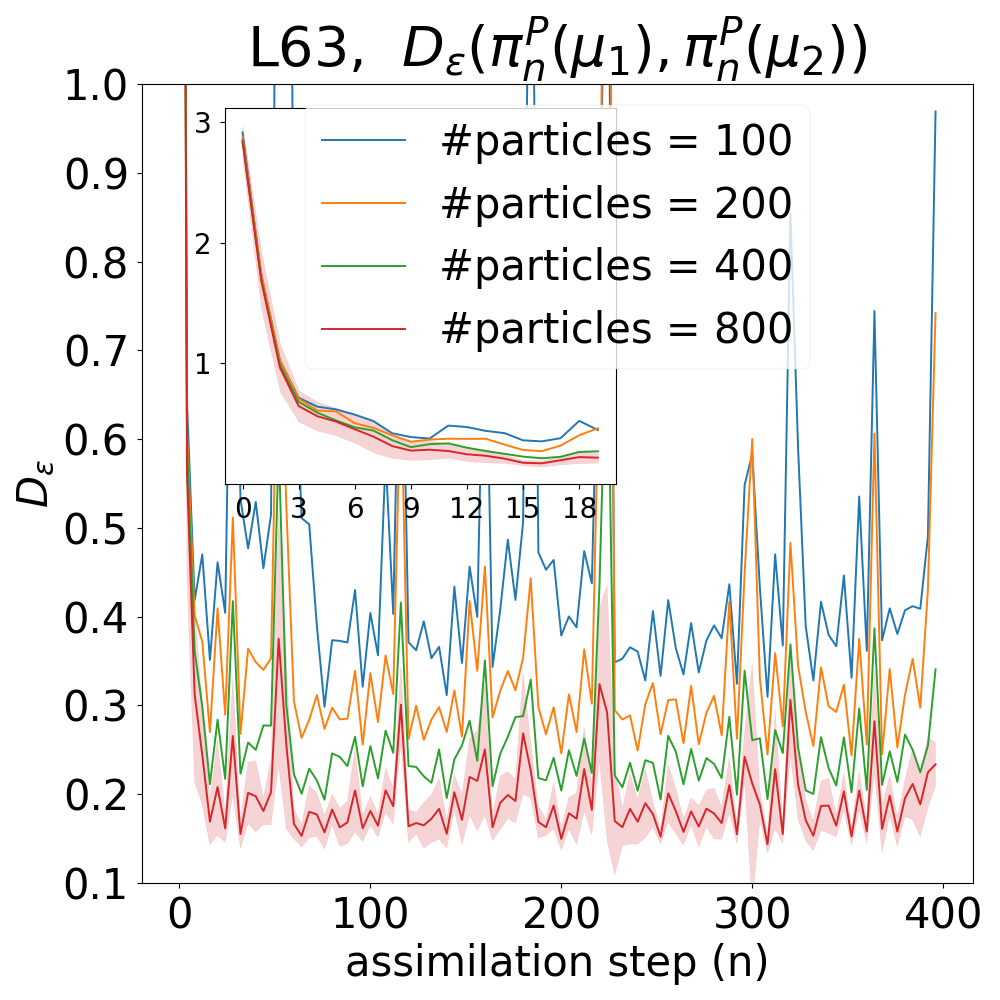
\includegraphics[width=0.2\textwidth]{stability/plots/figures-BPF-L63-0-dist_1_vs_2.png}} &
% {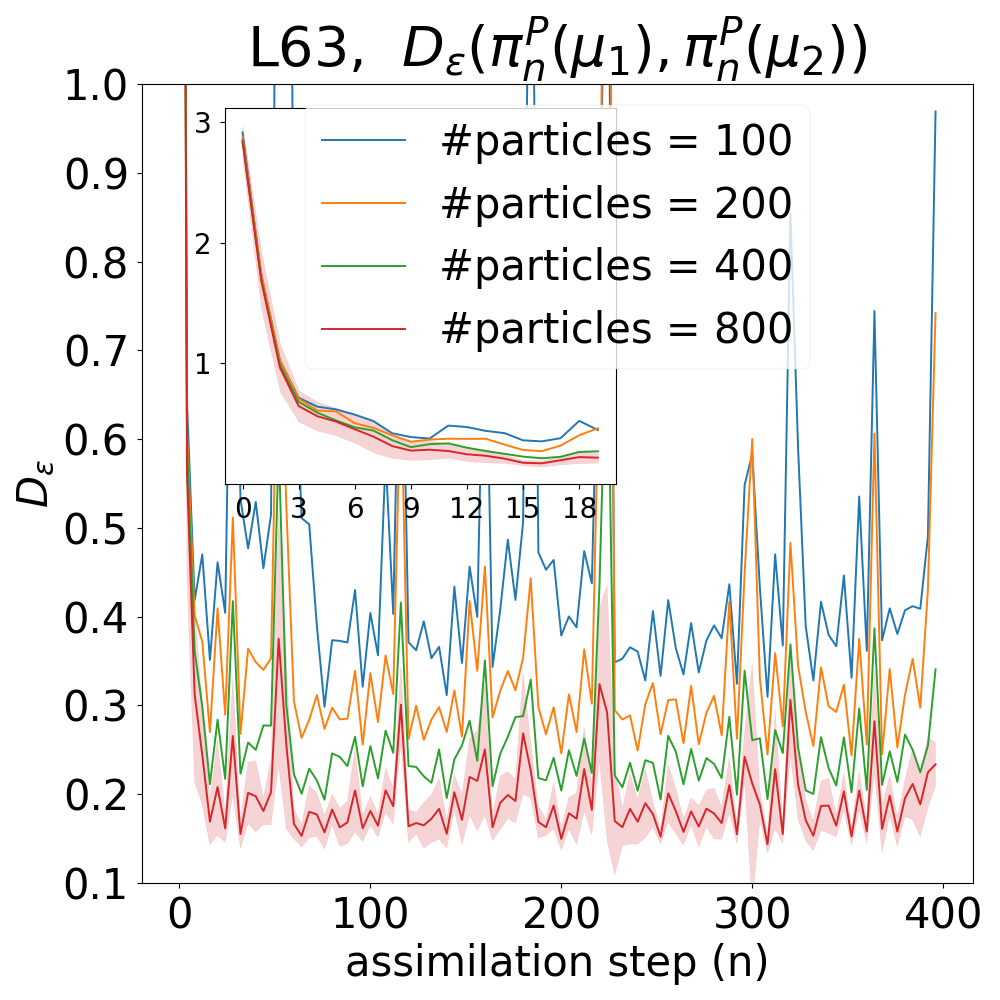
\includegraphics[width=0.2\textwidth]{stability/plots/figures-BPF-L63-0-dist_1_vs_2.png}} \\

% \end{tabular}
% \caption{Input Images}
% \end{figure*}





















%% -------------------------------------
\section{Discussion} \label{sec-disc--numerical-fs}
% \subsection{Explanation of the zero of the $S_\varepsilon$ algorithm}.
% \subsection{Explanation of the drop in $S_\varepsilon$ with increasing number of particles}

The main focus of this study was to develop a novel methodology to assess nonlinear filter stability using recently introduced techniques for calculating Wasserstein distances between distributions. We show that the particle filter and ensemble Kalman filter are stable when applied to a wide range of chaotic, deterministic dynamical systems, but the EnKF fails to capture the true filtering distribution.

We expect that the use of numerical algorithms for computing distances between the distributions will be a powerful tool for understanding nonlinear filters, leading to several avenues for further exploration. One direction of particular interest in earth sciences is to examine the relation between filter stability and the dynamical properties of the systems being observed.

%\addtolength{\textheight}{-12cm}
% This command serves to balance the column lengths
% on the last page of the document manually. It shortens
% the textheight of the last page by a suitable amount.
% This command does not take effect until the next page
% so it should come on the page before the last. Make
% sure that you do not shorten the textheight too much.

%% -------------------------------------
\section{Appendix: properties of Sinkhorn divergence} \label{sec-app--numerical-fs}
\begin{lem} If $\alpha, \beta, \alpha_m$ are probability measures on a compact set $\chi\subset\mathbb R^d$ then
\begin{align}
     & 0=S_\varepsilon(\beta, \beta)\le S_\varepsilon(\alpha, \beta)\\
     & \alpha=\beta\iff S_\varepsilon(\alpha, \beta)=0\\
     & \alpha_m\stackrel{\text{weak*}}{\longrightarrow}\alpha\iff S_\varepsilon(\alpha_m, \alpha)\to0
\end{align}
\begin{proof}
See Theorem $1$ in \cite{feydy2019interpolating}.
\end{proof}
\label{lem-prop--numerical-fs}
\end{lem}

\begin{lem}
If $\alpha_m, \beta_m, \alpha, \beta$ are probability measures supported on a compact set $\chi\subset\mathbb R^d$ such that $\alpha_m\stackrel{\text{weak*}}{\longrightarrow}\alpha$ and $\beta_m\stackrel{\text{weak*}}{\longrightarrow}\beta$ then $\lim_{m\to\infty}S_\varepsilon(\alpha_m, \beta_m)= S_\varepsilon(\alpha, \beta)$.
\label{lem-cont--numerical-fs}
\end{lem}
\begin{proof} Direct consequence of proposition 13 in \cite{feydy2019interpolating}.
\end{proof}
\begin{thm}
If $\alpha_m =\frac{1}{m}\sum_{i=1}^m\delta_{x^m_i}$ and $\beta_m=\frac{1}{m}\sum_{i=1}^m\delta_{y^m_i}$ are sampling distributions for the same underlying probability distribution $\mu$ which is supported on a compact set $\chi\subset\mathbb R^d$ then $\lim_{m\to\infty}S_\varepsilon(\alpha_m, \beta_m)=0$.
\label{thm-zero--numerical-fs}
\end{thm}
\begin{proof}
Direct consequence of lemmas \ref{lem-prop--numerical-fs} and \ref{lem-cont--numerical-fs}.
\end{proof}
\begin{thm}
If $\alpha_{m,n}, \beta_{m,n}, \alpha_n, \beta_n$ are random probability measures supported on a compact set $\chi\subset\mathbb R^d$ such that $\alpha_{m,n}\stackrel{\text{weak*}}{\longrightarrow}\alpha_n$ and $\beta_{m,n}\stackrel{\text{weak*}}{\longrightarrow}\beta_n$ as $m\to\infty$ and $$\lim_{n\to\infty}\liminf_{m\to\infty}\mathbb E [ D_\varepsilon(\alpha_{m,n}, \beta_{m, n})]=0$$ then, $\lim_{n\to\infty}\mathbb E[D_\varepsilon(\alpha_n, \beta_n)]=0$.\\
\begin{proof}
\begin{align*}
   &\lim_{n\to\infty}\mathbb E[D_\varepsilon(\alpha_n, \beta_n)]\\
    =& \lim_{n\to\infty}\mathbb E[\lim_{m\to\infty}D_\varepsilon(\alpha_{m,n}, \beta_{m,n})]\quad\text{by lemma }\ref{lem-cont--numerical-fs}\\
    \le&\lim_{n\to\infty}\liminf_{m\to\infty}\mathbb E[D_\varepsilon(\alpha_{m,n}, \beta_{m,n})]=0\quad\text{by Fatou's lemma}
\end{align*}
\end{proof}
\label{thm-stable--numerical-fs}
\end{thm}


%% -------------------------------------
% \section*{Acknowledgements} \label{sec-ack--numerical-fs}
% thanks for all the fish.

%% -------------------------------------



